\documentclass[article, nojss]{jss}
%\documentclass[article]{jss}
%% usepackage 
\usepackage[utf8x]{inputenc}
\usepackage[active]{srcltx}
\usepackage{amsmath}
%\usepackage{indentfirst}
\usepackage{amsfonts}
\usepackage{amssymb}
%\usepackage[round]{natbib}
\usepackage{ucs}
\usepackage{color}
%\usepackage{subfigure}
\usepackage{graphicx}
\usepackage{subcaption}
\usepackage{tikz}							% flow charts
\usetikzlibrary{shapes,arrows,calc}
\usepackage[inline,shortlabels]{enumitem}
\usepackage{calc}% http://ctan.org/pkg/calc
%
% \usepackage{Sweave}


%\VignetteIndexEntry{Simulation-based quasi-likelihood estimation with R}
%\VignetteDepends{}
%\VignetteKeywords{quasi-likelihood, simulation-based estimation, black box optimization, kriging-based metamodelling, cross-validation,uncertainty, R}
%\VignettePackage{qle}

%\DeclareMathOperator{\var}{var}
%\DeclareMathOperator{\cov}{cov}
\numberwithin{equation}{section}			% numbering acc. to sections
%
\author{Markus Baaske}
\title{Quasi-likelihood Estimation with \proglang{R}}
\Plainauthor{Markus Baaske}
\Plaintitle{Quasi-likelihood Estimation with R} 
\Shorttitle{Quasi-likelihood with \proglang{R}} 
%
\Abstract{
 We introduce the \proglang{R} package \pkg{qle} for simulation-based
 quasi-likelihood parameter estimation. We briefly summarise the basic theory
 of quasi-likelihood for our setting and outline the algorithmic framework of
 the proposed method. We focus on the general workflow using the
 package and present two introductory examples. Finally, we apply the method to an
 example data set from spatial statistics.
}
%
\Keywords{quasi-likelihood, simulation-based estimation,
black box optimization, kriging metamodel, cross-validation,
uncertainty, R}
\Plainkeywords{quasi-likelihood, simulation-based estimation,
black box optimization, kriging metamodel, cross-validation,
uncertainty, R}
%
\Address{
  Markus Baaske\\
  Faculty of Mathematics and Computer Science\\
  Friedrich Schiller University Jena\\
  07743 Jena, Germany\\
  Email: \email{markus.baaske@uni-jena.de}\\  
}
%
%% MATH -----------------------------------------------------------
\newcommand{\thetaOest}{\hat{\theta}_0}
\newcommand{\R}{\mathbb{R}}
\newcommand{\X}{\mathcal{X}}
\newcommand{\Sample}{\mathcal{S}}
\newcommand{\D}{\mathcal{D}}
\newcommand{\Rn}{\mathbb{R}^{n}}
\newcommand{\Rp}{\mathbb{R}^{p}}
\newcommand{\Rq}{\mathbb{R}^{q}}
\newcommand{\Pt}{\mathbb{P}_\theta}
\newcommand{\Et}{\mathsf{E}_{\theta}}  % \mathrm{E}_{\theta}
\newcommand{\var}{\mathsf{Var}_{\theta}} % \mathrm{Var}_{\theta}
\newcommand{\Ptheta}{\mathrm{P}_{\theta}}
\newcommand{\qle}{{\code{qle}}}
\newcommand\abs[1]{\left|#1\right|}
\newcommand{\norm}[1]{\left\lVert#1\right\rVert}
\newcommand{\subscript}[2]{$(\textrm{#1}\textrm{#2)}$}
\newcommand{\algstep}[2]{\textbf{#1} \textbf{#2}}
%
\newcommand{\help}[1]{\textcolor{red}{#1}}
\newcommand\numberthis{\addtocounter{equation}{1}\tag{\theequation}}
%BEGIN DOCUMENT
\begin{document}
% tikz settings
\tikzset{
  decision/.style={
    diamond, draw, text width=3em, text badly centered,
    node distance=3cm, inner sep=0pt
  },
  block/.style={
    rectangle, draw, text width=5em, text centered,
    rounded corners, node distance=3cm, minimum height=4em, inner sep=0.5pt
  },
  line/.style={
    draw, -latex'
  },
}
%
%\newcommand\linedatRIGHT[2]{% comment out this line-ending  
%  \par\noindent\rule{\textwidth}{1pt}\par\noindent
%  \textbf{Algorithm #1: #2}\par\noindent%
%  \leavevmode\noindent\rule[\fontcharht\font`M]{\textwidth}{0.5pt}  
%}
%
%\newcounter{AlgCount}
%
\section{Introduction}
The \proglang{R} package \pkg{qle} implements methods for parametric inference
for a generic class of estimation problems where we can at least simulate a
(hypothesized) statistical model and compute certain summary statistics of
the resulting model outcome. The method is an extended and modified
version of the algorithm proposed in \citet{Baaske2014}. The aim of this paper
is to present the algorithmic framework of our simulation-based quasi-likelihood
estimation (SQLE) approach for parametric statistical models. The method
employes the first two moments of the involved summary statistics by simulation and
constructs a quasi-likelihood approximation for estimating the statistical model
parameter.\par
%
We assume that, given the data, no closed-form expressions or direct computation
algorithms of likelihood functions or distribution characteristics, as functions of the
model parameter, are available. One may also be unable or reluctant to formulate
a likelihood function for complex statistical models. This precludes many standard
estimation methods, such as \emph{maximum likelihood} (ML) estimation,
typical Bayesian algorithms (including Markov-Chain-Monte-Carlo-type algorithms), or (generalized) least
squares (LS) based on exact distribution characteristics. In many settings, it is still conceptually
possible to consider some observed data as a realization of a vector of random
variables whose joint distribution depends on an unknown parameter. If a statistical model provides enough
information about the data generating process, we can think of it as partially
specifying some aspects of the distribution. However, it may be still possible to approximately compute
characteristics of the data as Monte Carlo estimates from computer simulations.
Such characteristics can be any sort of descriptive summary statistics which carry ''enough`` information
about the unknown dependency between simulated realizations and the model
parameter. Usually, these ''informative`` statistics are context-dependent and can be specifically tailored for the
setting of the parameter estimation problem under investigation.\par
%
\subsection{Quasi-likelihood approach}
If we could simulate the statistical model fast enough such that the Monte Carlo
error of the statistics becomes neglectable, a general approach for estimating
the model parameter would be to minimize some measure of discrepancy, i.\,e.
a criterion function, finding those parameters which lead to simulated
statistics most similar to the observed ones in the sense of a least squares, minimum contrast criterion,
or, more generally, estimating functions approach, see \citet{Godambe1991} and
also \cite{Jesus871}\footnote{For a more recent review on estimating functions
and its relation to other methods}.
The estimator of the true model parameter could then be found by a standard
numerical solver. However, complex statistical models usually require very
time-consuming, computationally intensive simulations and typically the Monte Carlo error cannot
be made small enough within a reasonable timeframe such that any direct
application of the above estimation approaches would become numerically infeasible.\par
%
Conceptually, our method is based on the class of linear estimating functions in
its most general form of minimum (asymptotic) variance unbiased estimation. We adapt the so-called
\emph{quasi-score} (QS) estimating function to the setting where generated
realizations of the statistical model can be characterised by a set of appropriately chosen summary
statistics. The derivation of the QS is part of the general approach of
\emph{quasi-likelihood} (QL) estimation, see \citet{ref:Heyde1997}, which subsumes standard parameter
estimation methods such as, for example, ML or (weighted) LS. The QL estimator
is finally derived from the solution to the QS equation (see Section \ref{sec:QL}).
As a common starting point the QS can be seen as a gradient specification
similar to the score vector in ML theory. If a likelihood is available, both
functions coincide and the score function from ML is an optimal estimating
function in the sense of QL.\par
%
Except in some rare cases, when expectations, derivatives thereof and variances
of the statistics are known at least numerically, any kind of criterion function derived from one
of the above criteria, including the QL approach, would lack a closed-form
expression and could only be computed slowly with substantial random error either due to the inherent
simulation variance or erroneous evaluation of the involved statistics. In fact,
nothing is said about a QL function in theory which could be employed as an
objective function for minimization in order to derive an estimate of the true
model parameter. Therefore, our idea is to treat such a function as a black box
objective function and to transform the general parameter estimation problem into a simulation-based
optimization setting with an expensive objective function. For this kind of
optimization problem it is assumed that derivative information is either not available or
computationally prohibitive such that gradient-based or Newton-type methods are not directly applicable.\par
%
\subsection{Background on black box optimization}
A general problem which holds both for finding a minimum of an expensive
objective function or a solution to the QS equation is to efficiently explore
the parameter search space when only a limited computational budget is
available for simulation. A suitable approach for this kind of problem relies on
the use of response surface models in place of the original black box function for optimization.
Examples include first-degree and second-degree (multivariate) polynomial
approximations of response functions, which are broadly used, for example, in
the \emph{response surface methodology}, see \citet{ref:Myers1995}. Another
approach includes the \emph{kriging methodology}
\citep[see, e.\,g.][]{ref:Sacksb1989,ref:Cressie1993,ref:Kleijnen2009} which treats the response of
an objective function as a realization of a stochastic process. The main idea is to start by evaluating
the expensive function at sampled points of a generated (space-filling)
experimental design over the whole parameter space.
Then a global response surface model is constructed and fitted based on the
initially evaluated design points and further used to identify promising points
for subsequent function evaluations. This process is repeated, now including the
newly evaluated points, for sequential updates of the response surface model.
In order to improve the model within subsequent iterations the aim is to select
new evaluation points which help to estimate the location of the optimum, that is, the unknown parameter
in our setting, and, at the same time, identifying sparsely sampled regions of
the parameter search space where little information about the criterion
function is available.\par
%
In this context, kriging has become very popular mainly for two reasons: first,
it allows to capture and exploit the data-inherent smoothness properties by
specifically tuned covariance models which measure the spatial dependency of the
response variable and, second, it provides an indication of the overall
achievable prediction or estimation accuracy. Almost all kriging-based global
optimization methods, such as the well-known \emph{Efficient Global
Optimization} algorithm by \citet{ref:Jones1998}, are based on the evaluation of
kriging prediction variances in one way or another\footnote{See \citet{ref:Jones2001} for a comprehensive overview
of kriging-based surrogate modelling.}. Although these models have been widely used
in the community of global optimization of expensive black box functions with applications to engeneering and
economic sciences these seem to be less popular in the context of
simulation estimation.\par
%
\subsection{Main contribution}
Opposed to the general framework of black box optimization, where
some scalar-valued objective function is directly constructed via
kriging, we propose the use of kriging models for each involved summary
statistic separately because, unlike the QS function itself, only the statistics can be estimated
unbiasedly from simulations. Based on these multiple kriging models we
construct an approximating QS estimating function and estimate the unknown model parameter as a root
of the resulting QS vector. Therefore, our main contribution is to combine the
QL estimation approach with a black box framework that allows to handle time-consuming simulations
of complex statistical models for an efficient estimation of the parameter of a
hypothesized true model when only a limited computational budget is available. Besides this, the use
of kriging models enables the estimation procedure to be guided towards regions
of the parameter space where the unknown model parameter can be found with some probability and
hence helps to save computing resources during estimation.\par
%
It is worth noting that there exist other \proglang{R} packages which make use
of the QL concept in one or another way. For example, the function \code{glm}
\citep{pkg:stats} for fitting a \emph{generalized linear model} is closely
related to the estimation theory by \citet{ref:Wedder1974} which is known
under the general term of \emph{quasi-likelihood methods}. From the viewpoint of
estimating functions this approach can be considered a special case of the
more general QL theory in \citet{ref:Heyde1997}. Also the package \code{gee}
\citep{pkg:gee} is made for a rather different setting which uses the
moment-based \emph{generalized estimating equations}, see \citet{ref:Liang1986}.
This package mostly deals with analysing clustered and longitudinal data which
typically consist of a series of repeated measurements of usually correlated
response variables. Further, the package \pkg{gmm} \citep{ref:pkgGMM} implements
the \emph{generalized method of moments} \citep{ref:Hansen1982} for situations
in which the moment conditions are available as closed-form expressions.
However, if the population moments are too difficult to compute, one can apply the
\emph{simulated method of moments} (SMM), see \citet{ref:McFadden1989}. The 
moment conditions are then evaluated as functions of the parameter by Monte
Carlo simulations. Also, the package \pkg{spatstat} \citep{pkg:spatstat}
includes a so-called quasi-likelihood method. However, the implementation is
specifically made for the analysis of point process models.\par
%
Our method is specifically designed to deal with situations where only a single
measurement (i.\,e. ''real-world`` observation or raw data) is available and
from which we can compute the (observed) summary statistics. To this end, we
assume that we can define and simulate a parametric statistical model which reveals
some information about the underlying data generating process. Then the
parameter of interest (under this model) is inferred from a solution to the QS equation based
on these statistics. The computational complexity of our method is, therefore,
mostly dominated by the effort of simulating the statistical model and evaluating the involved statistics.
The main aim of the package is to provide an efficient implementation for
generic parameter estimation problems which combines the involved statistics
into a tractable estimating function for simulation when no other types of
parametric inference can be applied.\par
%
The vignette is organized as follows. In Section \ref{sec:QL} we briefly
present the basic theory of QL estimation followed by an outline of the main
algorithm in Section \ref{sec:SQLE}. We discuss some extensions of our originally
proposed algorithm in Section \ref{sec:extent}. Finally, in Section
\ref{sec:Restim}, we provide some illustrative examples of a typical workflow of
using the package.
%

%
\section{Basic quasi-likelihood theory}\label{sec:QL}
In this section we sketch the main aspects of the general QL theory, see
\cite{ref:Heyde1997}. Let $X$ be a random variable on the sample space $\X$ whose
distribution $\Ptheta$ depends on the unknown parameter $\theta\in\Theta$ taking values
in an open subset $\Theta$ of the $q$-dimensional Euclidean space $\Rq$.
The goal is to estimate $\theta$ given the observed data $x=X$. We
assume that the family of models $\Ptheta$ is rich enough to characterise and distinguish
different values of the generative parameters. Let $T : \X\rightarrow \Rp$ with $p\geq q$ be a
transformation function of the data to a set of summary statistics and $y = T(x)$ is the respective
(column) vector of summary statistics. We follow the QS estimating function
approach to estimate $\theta$ by equating the QS
\begin{equation}\label{score}
  Q(\theta,y)=\left( \frac{\partial\Et[T(X)]}{\partial\theta} \right)^t \mathrm{Var}_{\theta}(T(X))^{-1}(y-\Et[T(X])
\end{equation}
to zero, where $(\cdot)^t$ denotes transpose, and, respectively, $\Et$ and
$\var$ denote expectation and variance w.r.t. $\Ptheta$.\par
%
For a fixed vector of summary statistics $T\in\R^p$ we focus on the function
$G(\theta,y)=y-\Et\left[T(X)\right]$ as a vector of dimension $p$, for which
$\Et\left[G\right]=0$ for each $\Ptheta$ and for which
the matrices $\Et\left[\partial G/\partial\theta\right]$
and $\Et\left[GG^t\right]$ are nonsingular.
The QS estimating function in \eqref{score} is the standardized estimating
function
\begin{equation}
 \tilde{G} = -\left(\Et\left[\frac{\partial G}{\partial \theta}\right]\right)^t (\Et\left[GG^t\right])^{-1}G
\end{equation}
for which the information criterion
\begin{equation}\label{information}
\mathcal{E}(G) = \Et\left[\tilde{G}\tilde{G}^t\right] = \left( \Et\left[\frac{\partial G}{\partial \theta}\right]\right)^t (\Et[GG^t])^{-1}
\left(\Et\left[\frac{\partial G}{\partial \theta}\right]\right)
\end{equation}
is maximized in the partial order of non-negative definite matrices among all
\emph{linear} unbiased estimating functions
of the form $A(\theta)(y-\Et\left[(T(X)\right]$, where $A(\theta)$ is any
nonsingular matrix. The information criterion in \eqref{information} is seen as generalization of the
well-known Fisher information since it coincides with the Fisher information in case a likelihood is available
such that $G$ equals the score function in ML theory. Then, in analogy to ML
estimation, the inverse of $\mathcal{E}(G)$ has a direct interpretation as the asymptotic variance of
the estimator $\thetaOest$. Moreover, $\mathcal{E}(G)$ might serve
as a measure of how much the statistics $T$ contribute to the precision of the
estimator derived from the QS equation. Under rather minor regularity conditions, the
estimator $\thetaOest$ obtained from solving the estimating equation $Q(\thetaOest,y)=0$ has minimum
asymptotic variance among all functions $G$ and consistency \citep[see,
e.\,g.][]{ref:Liang1995} is established due to the unbiasedness assumption of
the estimating equation in \eqref{score} which yields, in terms of its root, a
consistent estimator $\thetaOest$ even if the covariance structure is not correctly specified. The
information criterion in \eqref{information}, given a vector $T$ of summary
statistics, then reads
\begin{equation}\label{qi}
 I(\theta) = \var(Q(\theta,T(X)))= \left( \frac{\partial \Et\left[T(X)\right]}{\partial\theta} \right)^t \var(T(X))^{-1}
 \left( \frac{\partial \Et\left[T(X)\right]}{\partial\theta} \right),
\end{equation}
which we call \emph{quasi-information} (QI) matrix in what follows. In
particular, if we had an analytical or at least a numerically tractable form of the
involved expectations and variances, we could apply a gradient based method to
solve the QS equation similar to finding a root of the score vector in ML estimation. However, since closed-form
representations of expectations and variances are generally unavailable for
complex statistical models or prohibitive to compute we assume that we can only simulate realizations
of the random variable $\mathrm{X}$ under $\Ptheta$ at any $\theta\in\Theta$.\par
%
\section{Simulated quasi-likelihood estimation method}\label{sec:SQLE}
%
Let $Z\,:\,\Theta\rightarrow\R^p$ be a function of the model parameter
$\theta\in\Theta$ to the expected value of $T$, i.\,e. $Z(\theta)=\Et[T(X)]$,
and let $V(\theta)=\var(T(X))$ denote the variance of the statistics under
$\Ptheta$. Since we assume that we can only infer $T(X)$ by simulated
realizations of $X$ we treat $Z$ and $V$ as deterministic black box functions,
which could be very expensive to evaluate in practice. In order to compute the
QS function at $\theta$ the sample means of the statistics and the
variance $V$ are approximated by kriging models, denoted as $\hat{Z}$ and,
respectively, $\hat{V}$. Since both functions can only be evaluated with a
random error due to the simulation replications of the statistical model we
explicitly account for the resulting approximation error in the construction of the
QS function by adding the kriging prediction variances of the sample means of
the statistics (seen as a measure of predictive accuracy) to $\hat{V}$ as diagonal terms (see Section
\ref{subsec:varianceInter}). Then, the resulting approximation of the QS reads
\begin{equation}\label{approxscore}
  \hat{Q}(\theta,y)=\hat{Z}'(\theta)^t \hat{V}(\theta)^{-1}(y-\hat{Z}(\theta))
\end{equation}
given the observed statistics $Y=y$. Analogously, the approximation of the
information matrix in \eqref{qi} is
\begin{equation}\label{QI}
 \hat{I}(\theta) = \hat{Z}'(\theta)^t \hat{V}(\theta)^{-1} \hat{Z}'(\theta),
\end{equation}
where $\hat{Z}'\in\R^{q\times p}$ denotes the Jacobian (the matrix of partial
derivatives of $\hat{Z}$) which is numerically computed by finite differences
based on the kriging approximations of $Z$. The included diagonal terms
play the role of individual weights for the vector of contrasts
$y-\hat{Z}(\theta)$ in \eqref{approxscore} according to the predicted error
of $\hat{Z}$. Likewise, for the QI matrix in (\ref{QI}), the partial derivatives
of the kriging predictor $\hat{Z}$ are similarly weighted. Thus, the above QS
accounts for the noises due to the simulation replications of the
statistical model. Note that, compared to the typically high simulation effort
required to obtain an estimate of the statistics, the approximations of the QS function and QI
matrix can be computed inexpensively once the kriging models have been constructed. Besides
the kriging approach to approximate $V$ the package additionally provides other
types of variance average approximations, see \citet{Dryden2009}, including a
kernel-weighted verion based on the QI matrix.\par
%
Further, the SQLE method implements two criterion functions for estimation. The
first one is directly derived from quasi-likelihood theory. The so-called
\emph{quasi-deviance} (QD) is defined by
\begin{equation}\label{approxQD} 
  s(\theta) = \hat{Q}(\theta)^t \hat{I}(\theta)^{-1} \hat{Q}(\theta),
\end{equation} 
where we suppress the dependency on the observed statistics $y$ for
convienience. In particular, the QS and QD are considered as inexpensive approximations
of their respective counterparts if $T$ could be computed from $X$ under the
model $\Ptheta$ without error at any $\theta\in\D$. The QD - roughly speaking - measures the
''deviance`` of the QS vector from zero and thus provides a global view on the estimation
problem with the goal of solving the QS equation. Opposed to this, the
Mahalanobis distance (MD), which reads
\begin{equation}
  m(\theta)=\{y-\hat{Z}(\theta)\}^t\,\Sigma_{\theta}^{-1}\{y-\hat{Z}(\theta)\},
\end{equation}
where $\Sigma$ is a positive definite matrix, such as an estimate of the
asymptotic variance of $y$, has a direct interpretation as a (weighted or
generalized) least squares criterion depending on the employed type of variance
matrix approximation. It can be seen as a special case of SMM, where, in our
implementation, either $\Sigma_{\theta}=\Sigma(\theta)$ is evaluated as a function of $\theta$
(using Monte Carlo simulations) or considered as a ''constant`` estimate for
fixed $\theta$. In principle, both criterion functions can be used to guide the estimation procedure
towards a (possibly local) minimum or a root of the QS function. However, in
contrast to the QD, the gradient of the MD for constant $\Sigma$,
\begin{equation}
  m'(\theta)=\hat{Z}'(\theta)^t \Sigma^{-1}(y-\hat{Z}(\theta)),
\end{equation}
is readily available (ignoring irrelevant factors) and thus can be
used to minimize the criterion function by gradient based methods. This makes
the MD also desireable in terms of efficiency and numerical stability for local
searches. Obviously, in case the problem dimension equals the number of summary
statistics, i.\,e. $p=q$, both criterion functions coincide. Note that since the
MD can be subsumed under the general term of \emph{quasi-likelihood}, different versions
(see documentation) of the MD are implemented in the package mainly for two
reasons: first, the MD could be used as a preliminary step in order to identify suitable
starting points for parameter estimation and, secondly, to assess the
goodness-of-fit of the estimated model parameter.
%
\begin{figure}[!t]
\centering
\begin{minipage}[t]{0.75\textwidth} 
  \begin{tikzpicture}[auto]
    % Place nodes
    \node [block, text width=15em, minimum size=5em] (init) {Generate design,\\
    simulate and validate models,\\construct QS surrogate}; \node [block,
    below of=init,node distance = 2.5cm,text
    width=12em](minimize){Construct and minimize a criterion function};
    \node [decision,aspect=1.5, below of=minimize, node distance=2cm] (stop) {Stop?};
    \node [decision, aspect=1.5, below of=stop,node distance=2.5cm, text width=6.5em] (switch) {Local/Global phase?};
    \node [block, right of=switch, node distance=3.5cm] (global) {Global sampling};
    \node [block, left of=switch, node distance=3.5cm] (local) {Local sampling};
    \node [block, below of=switch, text width=10em, minimum height=3em, minimum size=2em, node distance=2cm] (update) {Simulate and update};
    \node [block, left of=stop, node distance=3.5cm, text width=5.5em] (final) {Check convergence and return};
    % Draw edges
    \path [line] (init) -- (minimize);    
    \path [line] (minimize) -- (stop);
    \path [line] (stop) -- node{no}(switch);
    \path [line] (stop) -- node{yes}(final);
    \path [line] (switch) -- (global);
    \path [line] (switch) -- (local);
    \path [line] (global) |- node[near start] {} (update);
    \path [line] (local) |- node[near start] {} (update);
    % Loop
    \path [line] (update) |- ($(update.south east) + (3.0,-0.5)$) |- (minimize);        
  \end{tikzpicture}
  \caption{Algorithmic strucure of function \code{qle}} 
  \label{fig:alg}
\end{minipage}
\end{figure}
%
\subsection{Algorithmic overview}
%
An outline of the algorithmic framework of our method is given in Figure
\ref{fig:alg}. The basic algorithm starts by generating an experimental design
of size $n_0$ of space-filling points, i.\,e. the parameters in our setting, and
evaluates the statistics at these initial design points by simulation. We say
that an \emph{evaluated point} is a point of the search space $\D$ where the statistical model
is simulated w.r.t. to this parameter or synonymously called ''point``. Based on
the same set of sample points and initially simulated statistics, the kriging models are separately
constructed for each statistic $T^{(j)}\in\R$, $j=1,\ldots,p$ so that
the algorithm needs to maintain and update $p$ kriging models simultaneously
each time a new evaluation point is added. Also, the user has the option to
analyse the initially generated design based on the chosen covariance structure in terms of its adequacy
for both the observed and simulated values of the statistics, the prediction
accuracy and the basic assumptions of the data phenomenon (see Section \ref{sec:design}).
Moreover, the prediction variance for each point is used to account for the
approximation error of the QS vector depending on the current iterate $\theta$ each time the algorithm
requests a new function value of the QS or the criterion function. In particular, finding a solution to
the subproblems in (\ref{QSE}) and (\ref{eOP}) also requires to evaluate either
of them.\par
%
During the main iteration the algorithm updates the QS approximation and the
criterion function based on newly evaluated design points, that is, we
sequentially select new parameters of the search space for simulating the statistical model
by the dual goal of improving the approximations and, at the same time,
narrowing the region of possible solutions of the QS function. To achieve this, the algorithm
is split into a local and global phase (see Section \ref{subsec:local} and \ref{subsec:global})
as shown in Figure \ref{fig:alg}, each using its own sampling and selection
criterion for new candidates and search methods to improve the current parameter estimate.
In particular, the global phase explores unvisited regions based on one of the
criterion functions where in some sense is evidence to suspect a global or local solution to the parameter
estimation problem. On the contrary, the local phase exploits promising local
regions for small values of the criterion function in the vicinity of an
approximate root or a minimizer. If the value of the criterion function drops below a user-defined tolerance
at some point, we immediately switch to the local phase and, otherwise, continue
with sampling in the global phase. Thus, the algorithm is allowed to dynamically switch the phases depending
on the number of successful iterations towards a potential parameter estimate.
The proposed sampling strategies and selection criteria ensure that the search space becomes overall densely
sampled if the algorithm is allowed to iterate infinitly often. Moreover, it
keeps a ballance between global and local search steps which is essential for the efficiency of the method
in practical applications and, at least in theory, guarantees to find a global
minimum.
%
\subsection{Approximately solving the quasi-score equation}
\label{subsec:qsSolve}
Througout this section we use the QD as the only criterion function for
monitoring the estimation. We aim on estimating $\theta_0=\theta_0(T)$ for 
given $T$ as the parameter of the hypothesized true model $\mathrm{P}_{\theta_0}$.
Using $\hat{Q}$ in (\ref{approxscore}) we deduce an estimate $\hat{\theta}\in\D$
from a solution to the approximating QS equation
\begin{equation}\label{QSE}
  \hat{Q}(\theta)\approx 0
\end{equation}
by a \emph{Fisher quasi-scoring iteration} \citep[see,
e.\,g.][]{ref:Osborne1992}. In practice, we observed that solving \eqref{QSE}
might cause numerical instabilities for small- or medium-sized sets of (initial) sample
points due to potential approximation inaccuracies of the resulting QS equation.
Therefore, even if there are no roots identifiable, we aim on searching for
at least an approximate (local) minimizer of one of the criterion functions and
then proceed using this last estimate. If we neither assume that equation
(\ref{QSE}) has a unique root nor that it exists, then, a common approach is to restrict
the estimation to ''plausible`` regions of the parameter space as to guarantee
the existence of a solution. Therefore, we define the parameter search space by
\begin{equation} 
  \mathcal{D}=\{\theta\in\Theta\;:\; \theta_l\leq\theta\leq\theta_u\}\subset\Theta,
\end{equation} 
where $\theta_l\in\Rq$ and $\theta_u\in\Rq$ denote the lower and
upper bounds, respectively, as simple bound constraints. In case of multiple
roots, restricting to reasonably chosen smaller subregions might also be a pragmatic
solution to distinguish between them. Another approach is given in Section
\ref{subsec:termCond}.\par
%
In our implementation, the quasi-scoring algorithm is defined as a projected
Newton-type iteration with the update
\begin{equation}
\begin{aligned}\label{qscoring}
  h & = \hat{I}(\theta)^{-1}\hat{Q}(\theta), \\
  \theta  & \leftarrow \mathcal{P}_D[\theta+\alpha h],  
\end{aligned}
\end{equation}
where $\mathcal{P}_D$ denotes the projection operator on $\D$ and $0<\alpha\leq
1$ is a step size parameter for the quasi-scoring correction $h\in\R^q$.
In contrast to the usual setting of ML estimation the quasi-scoring iteration
lacks explicit values of an objective function, monitoring the progress of the
iterates towards a root, because of the (in theory) left undefined
quasi-likelihood function. A natural way to measure the progress (adjusting the
correction $h$ and step length parameter $\alpha$ accordingly) is to use the QD as a monitor
function. Therefore, the purpose of the QD is twofold: on the one hand, it is used as
a surrogate objective function to monitor the root finding and guarantees the
existence of a global minimum over $\D\subset\Theta$. On the other hand, given
the observed statistics, we can also set up a hypothesis (see Section
\ref{subsec:testing}) of the estimated parameter to be the true one based on the
approximating QS and QD as a test statistic.\par
%
As a surrogate objective function, a global minimizer of the QD takes the QS closest
to zero (in the limit of a sequence of surrogate minimizations) and hence is
considered to be an estimate, not necessarily unique, of the unknown model parameter.
However, the quasi-scoring iteration might fail to converge in practice mainly for two reasons.
Besides pathological cases, for example, if no true root exists in $\D$, there are no
theoretically backed up tests of some sort of sufficient decrease condition (by
contrast to, for example, the Goldstein test or Armijo condition for ML estimation), which would
ensure global convergence to a root of the QS by a suitable line search
strategy. Therefore, we follow a hybrid search strategy in our implementation as
follows. If the quasi-scoring iteration fails, we switch to some
\emph{derivative-free optimization} method \citep[see, e.\,g.][]{ref:Conn2009} in order to approximately
solve the QS equation because we assume that derivatives of any of the involved
quantities of the QD are unavailable or computational prohibitive to obtain. In case of non-convergence,
we search for a minimizer of the (asymptotically) equivalent optimization
problem
\begin{align}\label{eOP}
   &\min s(\theta) \\
   &\text{s.t.}\; \theta\in\D.
\end{align}
However, the condition that $h$ is a descent direction, particularly for the QD
function, must be also checked to ensure a reasonable descrease after each updated
correction. In order to avoid additional expensive numerical computations of
function values and derivatives of the QS we implement this check as part of a line search
procedure using the simple condition
\begin{equation}\label{simple}
  s(\mathcal{P}_D[\theta+\alpha h]) < s(\theta) - \epsilon 
\end{equation}
of decreasing function values coupled with a backtracking algorithm, where
$\epsilon>0$ is used to ensure a minimum improvement in each iteration
similar to the \emph{sufficient decrease} condition in the Goldstein-Armijo
rule. Further, a backtracking line search is applied on the projection arc
$\mathcal{P}_D[\theta+\alpha h]$ and hence all iterates stay within the feasable
set $\D$.\par
%
\subsection{Estimating the error of the quasi-score approximation}\label{qsErr}
As a measure of accuracy of the QS approximation we transform the prediction
variances into an approximation error of the QS function. To this end, let
\begin{equation}
 \hat{B}_\theta=\hat{Z}'(\theta)\hat{V}(\theta)^{-1}\;\in\R^{q\times p}
\end{equation}
be a non-random weighting matrix given the data $Y = y$ w.r.t. to $\Ptheta$.
Then, assuming $\hat{B}_\theta$ and the \emph{statistical error} of the QS
function to be known, the QS approximation error reads
\begin{equation}\label{qsError}
 \hat{C}(\theta) =
 \textrm{Var}(\hat{B}_\theta(y-\hat{Z}(\theta)))=\hat{B}_\theta\hat{\Sigma}_K(\theta)\hat{B}_\theta^t\;\in\R^{q\times q},
\end{equation}
where the variance operation is w.r.t. to the distribution of the kriging
predictor $\hat{Z}$ and $\hat{\Sigma}_K$ denotes the diagonal matrix of kriging variances.
Since the inverse of the QI matrix serves as an estimated statistical lower
bound (like the Cram\'{e}r-Rao bound in ML theory) on the estimation error of $\hat{\theta}_0$,
we can compare the QS approximation error with the overall achievable accuracy
given by the QI matrix in \eqref{QI}. More specifically, if the largest
\emph{generalized eigenvalue} \citep[see, e.\,g.][]{ref:Golub1996}, say
$\lambda^{max}=\lambda^{max}(\theta)$, of these two matrices drops below some
limit $c\ll1$ such that
\begin{equation}
 \hat{C} \ll_L c\cdot\hat{I}
\end{equation}
holds in the Loewner partial ordering of non-negative definite matrices, we
say, that the QS approximation error is negligible compared to the predicted
error of $\hat{\theta}$. This can be seen as an indication that no further
benefit can be expected (from sampling new points) since we cannot get any better
in estimating the unknown model parameter given the simulated statistics at the
current design.
%
\subsection{Termination conditions}\label{subsec:termCond}
We define two types of termination conditions of the estimation procedure.
First, the \emph{statistical stopping conditions}, control the sampling
process and measure the level of accuracy of the QS approximation
and, secondly, the \emph{numerical conditions} which heuristically monitor the convergence
of the sequence of approximated roots of the QS or stationary points of the
criterion function. The algorithm stops sampling new evaluation points as soon as any
of these conditions hold and immediately terminates the estimation.\par
%
The statistical conditions measure the improvement of the QS approximation
achieved at iteration $n$, for example, the maximum variance of the estimated QS
approximation error
\[
    C^{max}_{n}=\max\{\text{diag}(\hat{C}_n)\},
\]
where $\hat{C}_n$ is defined in \eqref{qsError}. Since $C^{max}_n$ may strongly
fluctuate from one iteration to another due to the simulation variability,
we require to hold $C^{max}_n<C_{tol}$ for at least $N^C$ consecutive
iterations, where $N^C$ can be specified as an input argument to the algorithm.
Secondly, we compare the approximation error of the QS to its overall
achievable accuracy measured by the estimated QI matrix via the maximum generalized eigenvalue, say
$\lambda^{max}_{n}$. Then, if $\lambda^{max}_n<\lambda_{tol}$ holds for at least
$N^{\lambda}$ consecutive iterations we stop sampling. Both conditions relate to the fact of only approximately
knowing the QS vector based on the assumed stochastic model within a black box treatment of the
involved expectations and variances. We immediately stop the main iteration of
the allgorithm if any of the above termination condition holds.\par
% Numerical stopping conditions
In order to monitor the numerical convergence of the iterates, let
\[  
  Q_{max}(\theta) = \max_{1\leq i\leq q}\{|(\hat{Q}(\hat{\theta}))^{(i)}|\}
\]
denote the largest absolute deviation of the quasi-score vector from zero.
Numerical convergence, besides others, is signaled by the
conditions $Q_{max}(\theta)<\tau_0$ and $s(\theta)<s_{tol}$, where
$s_{tol}>0$ and $\tau_0>0$ are user-specified constants. For sufficiently
small constants $s_{tol}$, $\tau_0$ both conditions indicate an approximate
root of the QS vector. In particular, the latter also allows for a statistical
interpretation of the quasi-deviance as part of a Monte Carlo approach for
testing the goodness-of-fit of the statistical model w.r.t. the estimated parameter
$\hat{\theta}$ and provides us with another statistical stopping condition (see
Section \ref{subsec:testing}).
%
\section{Extensions and modifications}\label{sec:extent}
This section presents some extensions to the originally proposed QL approach in
\citet{Baaske2014}. Although it gives some insight in the algorithmic structure
of the method the section can be skipped.
%
\subsection{Select local evaluation points}\label{subsec:local}
Let
\begin{equation}\label{SS}
 \Sample_n=\{\theta_1,\ldots,\theta_n\}\subset\D.
\end{equation}
denote the sampling set of points of size $n$. The idea is to consider the
value of the QD as a test statistic and hence using it as a decision rule to
switch between the global and local phase of the algorithm. Suppose the
algorithm has either found a solution $\theta^*$ to the QS equation in (\ref{QSE}) or
a (local) minimizer of the QD in (\ref{eOP}) at some iteration $n\geq
n_0$ based on the current sampling set $\Sample_n$. If the value of the QD
function at $\theta^*$ is small compared to a user-defined upper bound, then
$\theta^*$ is considered as an estimate of the model parameter and the
algorithm stays in its local phase exploring the local vicinity for further refinement
of $\theta^*$. During both phases the algorithm samples new points of
$\D$ which we call \emph{candidates} for evaluation. In particular, during the
local phase the algorithm randomly generates candidate points (without
evaluating them) $\theta\in\Omega^l_n$, where $\Omega^l_n$ denotes the set of local
candidates, according to a multivariate normal distribution with mean equal to the current
minimizer and variance equal to the inverse information matrix in
\eqref{QI}. Otherwise, the algorithm is in its global phase.\par
%
In order to measure the potential benefit of adding some point out of all
candidates in $\Omega^l_n$ during the local phase of the algorithm we
adapt the idea proposed in \citet{ref:Regis2007} to our setting. Let
\begin{equation}
\bar{s}_n(\theta) := \hat{Q}_n(\theta)^t \hat{C}_n(\theta)^{-1} \hat{Q}_n(\theta)
\end{equation}
denote a \emph{modified} version of the QD in \eqref{approxQD}, that is, the
quasi-information matrix replaced by the error matrix of the QS vector (see
Section \ref{qsErr}) at iteration $n$. Then
\begin{equation}\label{stilde}
 \tilde{s}_n(\theta) = 
  \begin{cases} 
   \frac{\bar{s}_n(\theta)-\bar{s}^{\textrm{min}}_n}{\bar{s}^{\textrm{max}}_n-\bar{s}^{\textrm{min}}_n}
   & \textrm{if } \bar{s}^{\textrm{min}}_n\neq \bar{s}^{\textrm{max}}_n \\ 1 &
   \textrm{otherwise}.
  \end{cases}
\end{equation}
denotes its normalized value where the minimum and maximum
of the modified QD is given as
$\bar{s}^{\textrm{min}}_n=\min\{\bar{s}_n(\theta)\,:\,\theta\in\Omega^l_n\}$ and, respectively,
$\bar{s}^{\textrm{max}}_n=\max\{\bar{s}_n(\theta)\,:\,\theta\in\Omega^l_n\}$.
Also let
\begin{equation*}
 \Delta_n(\theta)=\min_{\tilde{\theta}\in\Sample_n} ||\theta-\tilde{\theta}||_{2}  
\end{equation*}
denote the minimum distance of points $\theta\in\D$ to all previously sampled
points belonging to $\Sample_n$. Then, the maximum and minimum values of these
distances over all pairs of $n$ points in $\D$ are given by
\begin{eqnarray*}
  \Delta^{\textrm{min}}_n & = & \min\{\Delta_n(\theta)\,:\theta\in\mathcal{D}\},\\
  \Delta^{\textrm{max}}_n & = & \max\{\Delta_n(\theta)\,:\theta\in\mathcal{D}\}.     
\end{eqnarray*}
Again, we normalize the distances $\Delta_n(\theta)$ to the interval $[0,1]$ by
\begin{equation*}
 w_n(\theta) = 
  \begin{cases} 
   \frac{\Delta^{\textrm{max}}_n-\Delta_n(\theta)}{\Delta^{\textrm{max}}_n-\Delta^{\textrm{min}}_n}
   & \textrm{if } \Delta^{\textrm{min}}_n\neq \Delta^{\textrm{max}}_n \\ 1 &
   \textrm{otherwise}.
  \end{cases}
\end{equation*}
Then, the next point which minimizes 
\begin{equation}\label{scoreCrit}
  v_n(\theta)=\gamma^l_j \tilde{s}_n(\theta)+(1-\gamma^l_j)w_n(\theta)
\end{equation}
is added to $\Sample_n$ for evaluation, where $1\leq j\leq r$ and
$\theta\in\Omega^l_n$. For given weights $0\leq \gamma^l_1,\ldots,\gamma^l_r\leq 1$ we refer to
$\Gamma^l=\langle \gamma^l_1,\ldots,\gamma^l_r\rangle$ as a \emph{local weight
pattern} of \emph{cycle length} $r$. The weights define the degree of
global/local selection of new evaluation points. More specifically, this 
local selection criterion results in minimizing the modified QD if
$\gamma^l_r=1$ and otherwise, if $\gamma^l_1=0$, maximizing the minimum distance to all other sampling
points from $\Sample_n$. Cycling through $\Gamma^l$ selects new points which
have relatively low values of the modified QD and become more distant to previously sampled points
for increasing weights. Based on the newly simulated statistics at the selected
point the kriging models are updated and thus the QD approximation is further
improved as represented in the last block at the bottom of Figure \ref{fig:alg}. The process is
iterated until any stopping condition (see Section \ref{subsec:termCond})
is satisfied. The resulting solution based on the final approximation of the QS
and QD is taken as an estimate of the unknown model parameter.\par
%
Besides a pre-specified weight pattern the algorithm also includes an automated
adjustment of the weights according to the progress of the iterates and achieved
accuracy of the QS approximation. By this, we intend to faciliate convergence
of our method. We say that the current local phase at iteration $n$ was
\emph{successful} in case the following conditions hold
\[
 s_n<s_{n-1},\; \lambda^{max}_n<\lambda^{max}_{n-1},\; C^{max}_n<C^{max}_{n-1}
\]
and \emph{failed} otherwise. We record the number successful and failed local
phase iterations and as soon as the above conditions hold for a certain
number of consecutive iterations the weights are increased by a user-defined
scalar value. Otherwise the weights are decreased in the same way. We follow the
reasoning that for a sequence of increasing weights the estimated accuracy of
sequential QS approximations improves locally and thus can be trusted more and
more so that new evaluation points are selected in the vicinity of the current
best estimate. This forces the algorithm to select and evaluate new points more close
to the current best estimate in order to reduce the (approximately pointwise)
simulation variability of the statistics and hence to improve the accurary of
the QS at this point. Otherwise, for descreasing weights the algorithm
tends to select points in between previously sampled points due to the higher
weighted minimum-distance term in (\ref{scoreCrit}). This implies a less
beneficial impact on imroving the QS approximation by previously evaluated
points and, therefore, the algorithm follows the ''infill`` strategy.\par
%
As another local selection criterion we propose a distance-weighted
version of the \emph{trace criterion}, see \citet{ref:Puk2006}. The next sample
point is selected as
\[
  \theta_{n+1} = \text{arg}\max_{\theta\in\Omega^{g}_n}w_n(\theta) \frac{1}{q}tr\{\hat{C}_n(\theta)\},
\]
where $tr\{\cdot\}$ denotes the trace of a matrix. The criterion mostly selects
points in relatively unexplored regions of the parameter space with a
relatively high approximation error of the QS function. However, potential
candidates more close to already sampled points get smaller weights which prevents
the algorithm from clustering too much around previously sampled points.
This strategy might be useful in case we rapidly want to improve the quality of the QS
approximation within a few additional simulations of the statistical model
followed by a root finding local search. Note that this selection criterion has
a tendency to sample points at the ''border`` of the sample space first due
to the extrapolation properties of the kriging estimators.\par
%
\subsection{Select global evaluation points}\label{subsec:global}
The main goal of the global phase of the algorithm is to sample new
evaluation points which can be far away from previously sampled points and widely
spread over the entire search space. While the global sampling can improve the
QS approximation at any point finding possible solutions anywhere in the search
space the local sampling procedure essentially is a local search algorithm since it only
explores a local region in the vicinity of the estimated solution and improves its
predicted location. Therefore the local phase cannot be used for global
optimization alone. The main reason why it is necessary to use a global sampling procedure
is that we need to investigate different local regions where low values of the
QD could turn out to be approximate solutions and the other way round, approximate
roots could vanish while new sample points are evaluated. The two sampling
procedures differ in the generation of candidate points and also in the selection of
weights to achieve a balance between global and local search which is a basis
for efficient global optimization.\par
%
Let $\Omega^g_n$ be the set of uniformly distributed global candidate points
over $\D$. New evaluation points are selected from $\Omega^g_n$ based on a
weighted distance measure, where candidate points with low predicted QD value
obtain higher weights. In this way, the QD serves as a monitor function to
indicate promising and relatively unexplored regions. We use a strictly
positive weight function, that is, $u_n(\theta)>0$ for all $\theta\in\Omega^g_n$,
which never fully ignores any region of the search space. The form of the
weight function, which also can be found in \citet{ref:Jakobsson2010} as part of
a different selection criterion, is defined by
\begin{equation}
 u_n(\theta) = \exp\Big\{ -\gamma \, \tilde{s}_n(\theta) \Big\},
\end{equation}
where $0\leq\gamma<\infty$ denotes a weight parameter and $\tilde{s}_n$
denotes the normalized QD in \eqref{stilde}.
We select the candidate which maximizes the weighted minimum distance
\begin{equation}\label{globsamp}
  \theta_{n+1} = \text{arg}\max_{\theta\in\Omega^{g}_n} u_n(\theta)\Delta_n(\theta)
\end{equation}
for the next evaluation. The weight parameter controls the balance between a
local and more global selection of new points and the weight function is
constructed such that, if $\gamma=0$, then $u_n=1$ holds for all $\theta\in\Omega^g_n$.
In this case, the value of the QD is ignored and the next sample point maximizes
the miniumum distance, i.\,e. in a space-filling manner, from all other samples
of $\Sample_n$. For parameter values $\gamma\rightarrow\infty$, candidate points with relatively
low values of the QD obtain much higher weights and hence we more and more trust the
approximation of the QD. As in the local phase, we also intend to balance the
sampling and, therefore, switch between a local and more global sampling by
iterating the weight parameters $\gamma\in\Gamma^g$ in the same way as in
\eqref{scoreCrit}. In contrast to the local selection rule there is no automated
update of these weights implemented.\par
%
Note that, besides the above infill selection criteria, which keep a
balance between global and local search steps, we implicitly account for the
approximation error of statistics in both criterion functions. As a result, even
if the chosen weights lead to a pure minimization of one of the criterion functions, new candidates
make a compromise between being a local minimizer and improving the accuracy of
the QS approximation. Thus, pure local candidates still improve the QS function w.r.t. its approximation error.
%
\subsection{Variance matrix estimation}\label{subsec:varianceInter}
Besides the kriging approach to approximate the variance matrix proposed in
\citet{Baaske2014} the package additionally offers a (weighted) average
approximation. Let $\theta_1,\ldots,\theta_n$ belong to the
current sample set $\Sample_n$ at iteration $n$ of the algorithm. The idea
is to estimate $V(\theta)$ for $\theta\in\D$ by averaging over the	
simulated sample of covariance matrices $V(\theta_1),\ldots,V(\theta_1)$. To this end,
we estimate $V(\theta)$ by the mean sample covariance matrix $E(V_i)$, see
\citet{Dryden2009}, of sample matrices $V_i=V(\theta_i)$, $i=1,\ldots,n$,
with an assumed i.i.d. scaled Wishart distribution for $V_i=V(\theta_i)$. The package includes
two basic types of sample average estimators. The first one is based on the
Cholesky reparametrization, i.\,e. matrix decomposition, of sample covariance
matrices, wich reads
\begin{equation}\label{L}
 V=LL^{t} \quad \textrm{with} \quad L=\textrm{chol}(V)\in\R^{p\times p},
\end{equation}
where $L$ is a lower triangular matrix with real and positive diagonal elements.
Then, an estimator of $E(V_i)$ is given by
\begin{equation}\label{VC}
 \bar{V}_{C} = \bar{L}\bar{L}^t, \textrm{ where} \quad \bar{L} = \frac{1}{n}\sum_{i=1}^n L_i
\end{equation}
with $L_i=L(\theta_i)$.
Alternatively, an estimator based on the matrix logarithm \citep[see,
e.\,g.][]{ref:Golub1996}, i.\,e. \mbox{$\log V=U(\log\Lambda)U^t$}, of sample
covariance matrices $V=U\Lambda U^t$ using the common spectral decomposition with an orthogonal
matrix $U$, can be obtained by
\begin{equation}\label{VL}
 \bar{V}_L = \exp\Bigg\{\frac{1}{n}\sum_{i=1}^n \log V_i \Bigg\}.
\end{equation}
\citet{Dryden2009} empirically shows that both estimators perform well
in a series of test problems.\par
However, a locally weighted version of the estimated mean sample covariance
matrix in (\ref{VC}) or (\ref{VL}) might be preferable in case of an already
available approximate root $\hat{\theta}_0$ by $Q(\hat{\theta}_0)\approx 0$
in (\ref{score}). Therefore, we apply a Nadaraya-Watson \emph{kernel-weighted
average}, see \citet{Qi2007}, for both types of averaging matrices. In analogy
to (\ref{VC}), this leads to the estimator
\begin{equation}\label{wVC}
 \tilde{V}_C=\tilde{L}\tilde{L}^t\quad \textrm{with}\quad \tilde{L} = \frac{\sum_{i=1}^n
 K(\theta_i,\hat{\theta}_0) L_i}{\sum_{i=1}^n K(\theta_i,\hat{\theta}_0)},
\end{equation}
where $K$ is the multivariate Gaussian kernel
\begin{equation}\label{kernel}
  K(\theta,\hat{\theta}_0) = \exp\bigg\{ -(\hat{\theta}_0-\theta)^t
  W(\hat{\theta}_0)^{-1}(\hat{\theta}_0-\theta)\bigg\}
\end{equation} 
and $W=\hat{I}^{-1}$ is the weighting matrix.
Likewise, the weighted version of (\ref{VL}) reads
\begin{equation}\label{wVL}
 \tilde{V}_L=\exp\{\bar{M}\}\quad \textrm{with}\quad \bar{M} = \frac{\sum_{i=1}^n
 K(\theta_i,\hat{\theta}_0) (\log V_i)}{\sum_{i=1}^n K(\theta_i,\hat{\theta}_0)},
\end{equation}
where $\exp\{\cdot\}$ denotes a matrix exponential. Moreover, the choice of
kernel function is motivated by the idea that the asymptotic distribution of $(\hat{\theta}-\theta)$
is (under conditions ensuring asymptotic normality of the statistics, like ergodicity and sufficient
regularity) normal with variance $I^{-1}$, see \citet[sect.~4.3]{ref:Heyde1997}.
Note that the weighted variance matrices in (\ref{wVC}) and (\ref{wVL}) depend on an approximate root
$\hat{\theta}_0$ in (\ref{kernel}), which also must be given in order to compute the variance estimate.\par
%
Finally, to account for the simulation error of $\hat{Z}$ we add $\hat{\Sigma}$
in (\ref{qsError}) to the variance matrix average approximation by
\begin{equation}\label{modVar}
  \hat{V}(\theta) = V^* + \hat{\Sigma}(\theta),  
\end{equation}
where $V^*$ stands for any of the above types of matrix estimates
and $\hat{\Sigma}$ denotes the diagonal matrix of prediction variances of
$\hat{Z}$. Alternatively, a cross-validation approach (see Section
\ref{subsec:altVar}) can be applied to estimate the prediction variances. The same
strategy is used for the originally proposed kriging approach to approximate the
variance matrix in \cite{Baaske2014}.
%
\subsection{Alternative estimation of prediction errors}\label{subsec:altVar}
% 1. Ziel: Modellvalidierung und Unsicherheit
The use of kriging models allows the construction of relatively inexpensive
approximations of the sample means of statistics compared to the effort required
for evaluating the statistics based on the statistical model simulations only.
In addition, we have some readily available indication of prediction accuracy at unsampled points
measured by the kriging predictor variances. However, the main drawback of considering
the kriging variance as a measure of prediction uncertainty stems from its
inherent independence of the observed values as part of the prediction. The
kriging variance, therfore, is strongly related to the spatial configuration
(locations and interdistances) of sampling points and thus should not be viewed as an predictor's
precision but rather as an ``precision indicator'' as argued in
\citet[sect.~3.4.4]{ref:ChilesDelfiner1999}. Moreover, the kriging variance is directly
affected by the subjectively chosen covariance structure which is nearly impossible to be
correctly specified in practice and, therefore, simply set beforehand
assumed to be known without error. Practically, the kriging predictor is
obtained by simply plugging-in the estimated parameters of the covariance model
for the observed data which formally leads to a conditional predictor variance.
Then, for instance, the kriging variance might not reflect the total amount of uncertainty
in predicting values at unsampled points and is often underestimated
\citep[see][for a comprehensive discussion]{ref:Marchant2007}. Consequently, any algorithm
for parameter estimation which relies too much on prediction variances could be seriously
misleaded.\par
%
For this reason, the package also includes an alternative strategy to predict
the actual error. We use a cross-validation (CV) approach to estimate the degree
of dependence between the spatial location of sampled points including the response
of the statistical model, i.\,e. the value of a statistic, and its impact on the level
of accuracy for predicting at new points. In order to assess the validity and
uncertainty of kriging approximations we consider the \emph{jackknife variance}
(based on a specific CV approach tailored for simulation-based kriging) as
proposed in \citet{Kleijnen2004a} as well as the estimation of the
\emph{root mean squared error} (RMSE), see \citet{Jin2002}, including an option
to control the computational effort. Note that we consider the prediction variance
based on kriging and CV as complementary to one another and point out that the computation
of both types does not require additional simulations of the statistical
model.\par
%
Let
\begin{equation} 
  \mathcal{Y}_n=\{\bar{y}_1,\ldots,\bar{y}_n\}  
\end{equation}
denote the set of simulated sample means of statistics at parameters
$\theta\in\Sample_n$ for $i=1,\ldots,n$. Given the sampling set $\Sample_n$ as in (\ref{SS})
we eliminate the $i$th element of $\Sample_n$ and obtain the CV sample $\Sample_n^{(-i)}$ of size $n-1$.
For completeness we present the formulas for the \emph{jackknife's
pseudo-value}, \emph{jackknife variance} and refer to \citet{Kleijnen2004a} for
a detailed description. The jackknife's pseudo-value for the kriging predictor
$\hat{Y}$ at some parameter $\theta$ is treated as a (kriging) mean based on the
original sample $\Sample_n$ defined by
\begin{equation}\label{pseudo}
  \tilde{y}_{i}(\theta) = n\hat{Y}(\theta)-(n-1)\hat{Y}^{(-i)}(\theta)\,\in\R\,,
\end{equation}
where $\hat{Y}^{(-i)}(\theta)$ denotes the response of the kriging model at
$\theta$ with the simulated data $(\theta_i,\bar{y}_i)$ removed from
$\Sample_n\times\mathcal{Y}_n$ for $i=1,\ldots,n$.
From these values the jackknife variance at the sample point $\theta$ is
estimated by the usual sample variance
\begin{equation}\label{jackVar}
  \tilde{\sigma}^2_{CV}(\theta) = \frac{1}{n(n-1)}\left(\sum_{i=1}^n(\tilde{y}_{i}(\theta)-\overline{\tilde{y}}(\theta))^2 \right)
  \quad\textrm{with}\quad\overline{\tilde{y}}(\theta)=\frac{1}{n}\sum_{i=1}^n \tilde{y}_{i}(\theta). 
\end{equation}
As another measure to assess the kriging model fidelity, for example, to
validate different realizations of initial sampling designs, we can use
\begin{equation}\label{rmsecv}
 RMSE(\theta) = \sqrt{\frac{1}{n}\sum_{i=1}^n \left(\hat{Y}^{(-i)}(\theta)- \hat{Y}(\theta)\right)^2}
\end{equation}
at the sample point $\theta$ based on the CV approach mentioned before. Note
that the calculation of the jackknife variance in (\ref{jackVar}) and RMSE for various
unsampled points in a sequential selection procedure requires the re-estimation
of covariance model parameters for each sampling set $\Sample_n^{(-i)}$.
In practice, this could be prohibitive as the number of overall sampling points
grows during the estimation procedure. The high computational effort is mainly due
to the number of REML estimations which must be carried out for $n$ covariance
models each based on $n-1$ sampling points. If $n$ becomes large, then the
pseudo-values in (\ref{pseudo}) might not much differ anymore which would lead to variances
mostly due to simulation error. Therefore, we also can apply a \emph{block
jackknife} scheme \citep[see, e.\,g.][and references therein]{Shao1995} in
addition to the \emph{delete-1 jackknife} method for large $n$ and proceed as
follows. We limit the number $n_c$ of covariance models still to fit,
i.\,e. the number of subsets of $\Sample_n$, by $n_c\leq n$ with maximum $k$ sampling points
deleted from $\Sample_n$ for each covariance model fit such that $n=n_ck$.
Then, we define the pseudo-values in analogy to (\ref{pseudo}) as
\begin{equation}\label{pseudonc}
 \hat{y}_{i}(\theta) = n_c\hat{Y}(\theta)-(n_c-1)\hat{Y}^{(-i)}(\theta),
\end{equation}
where the index $i$ with $1\leq i\leq n_c$ now refers to the block $i$, possibly
being a one-element (if $k=1$), which consists of $k$ sample points to be
removed from $\Sample_n$ for the purpose of covariance fitting and construction of the
corresponding kriging predictors $\hat{Y}^{(-i)}$. Then, we proceed as in
(\ref{jackVar}) or (\ref{rmsecv}) with $n$ replaced by $n_c$. Note that this case also
includes the delete-1 jackknife method and thus we will always refer to $n_c$ as
the maximum number of blocks. Moreover, in \citet{Meckesheimer2002} the
authors report that choosing $k=0.1n$ or $k=\sqrt{n}$ for the RMSE in (\ref{rmsecv}) provides good error
estimates when kriging models are used for prediction and design analyses.
Therefore, we choose $k$ proportional to the overall number of sample points $n$
currently reached and dynamically increase $k$ in a step by step manner if $n$ grows beyond
a pre-defined upper limit during the estimation procedure. Nevertheless, using
prediction variances based on CV instead of kriging is obviously computationally more demanding
since, despite of the strategy explained above, additional covariance models have to be estimated
and iteratively updated during the overall estimation procedure. This is the
price the user has to pay for a possibly more realistic treatment of prediction uncertainty which
is likely to result in a more robust final model parameter estimate. Unless the
structure of the general estimation problem is relatively simple we recommend to use the CV based approach.
%
\subsection{Initial design validation}\label{sec:design}
In order to contruct a reasonable global approximation model of the QD we show how
to assess the predictive quality and goodness-of-fit of a pilot design based on
each kriging model separately. The idea is to use the same type of prediction
variance, e.\,g. by kriging or CV, for the analysis of the initial design and
later on during the sequential candidate selection strategy. This ensures a
consistent treatment of selecting a new candidate point without spending too much effort on
the calculation of prediction variances or performing additional
simulations.\par
%
The most commonly applied concepts are based on kriging prediction variances and resampling methods
such as bootstrapping and cross-validation. The reader is refered to
\citet{ref:Sacksb1989} for an overview of various strategies empirically investigated in the context
of simulation-based optimization. Although, in principle, automated procedures
are available to choose and augment a design optimally for a global
metamodelling \citep[see e.\,g.][sect.~6]{mueller2001} we rather focus
on which type of prediction variance best reflects the true variability of predictions and
hence the statistical model. The reasoning is, that this choice has a certain impact on the
efficiency of the sampling process towards a reasonable estimate of the model parameter, because
the prediction variance is directly involved in the selection of new evaluation
points based on one of the available criterion functions. Besides this, a
two-stage design optimization criterion, such as \emph{integrated mean squared error}
\citep[see, e.\,g.][]{ref:Sacksa1989}, could be applied.\par
%
Although, our estimation method does not require a specific initial design (as
long as it inherits a space-filling property) a carefully chosen pilot design
usually results in faster convergence of the algorithm and a less number of
additional sample points. Instead of using CV for estimating the prediction
variances at candidate points (see Section \ref{subsec:altVar}) here we use the
CV approach to empirically validate the adequacy of the kriging model, for example, assumptions
either about the employed class of covariance models and the involved
fitted parameters, the initial sampling size used to build the kriging model or
about the variability of simulated statistics over the entire parameter space.
To this end, we modify the CV approach in \citet[sect.~11]{ref:Wackernagel2003}
as follows.\par
%
Let $\hat{Y}^{(-i)}(\theta_{i})$ be the value of the kriging
predictor at $\theta_i\in\Sample_0$ with the simulated data
$\left(\theta_i,\bar{y}_i\right)$ removed from $\Sample_0\times\mathcal{Y}_0$.
If the average CV error (ACVE) defined by
\begin{equation}\label{ACVE}
\textrm{ACVE}=\frac{1}{n}\sum_{i=1}^n
\left(\hat{Y}(\theta_i)-\hat{Y}^{(-i)}(\theta_i)\right) \approxeq 0\,,
\end{equation}
where $\hat{Y}(\theta_i)$ denotes the prediction including the
full sample set $\Sample_0$, $i=1,\ldots,n$, then we say that there
is no apparent bias in predicting at left-out sample points. Otherwise a value 
which significantly distinguishes from zero could represent (systematic) over-
or underestimation of the kriging prediction variances by the corresponding
predictor. Due to the simulation error of evaluating the statistics $Y$ we
estimate the observed value $\bar{y}_i$ by the noise-free response, see
\citet[][sect.~3.7.1]{ref:ChilesDelfiner1999}, of the kriging predictor in
(\ref{ACVE}) instead of the simulated statistics itself as proposed in
\citet{ref:Wackernagel2003}.\par
%
Also, the magnitude of the \emph{mean squared cross-validation errors} (MSE) of
predicting the statistics gives an impression on the sensitivity of the corresponding
statistic $Y$ leaving out a sample point $i$ of the design for estimating the
corresponding sample mean value
\begin{equation}\label{MSE}    
  \textrm{MSE}=\frac{1}{n}\sum_{i=1}^n
  \left(\hat{Y}(\theta_i)-\hat{Y}^{(-i)}(\theta_i)\right)^2.
\end{equation}
Further, to compare the magnitudes of the actual CV error with the one induced
by the corresponding kriging model we define the squared \emph{standardized
cross-validation error} (SCVE), which reads
\begin{equation}\label{SCVE}    
  \textrm{SCVE}(\theta_i)=\frac{\left(\hat{Y}(\theta_i)-\hat{Y}^{(-i)}(\theta_i)\right)^2}{(\hat{\sigma}^2)^{(-i)}(\theta_i)}\,,
\end{equation}
where $(\hat{\sigma}^2)^{(-i)}$ denotes the kriging variance with the data pair $(\theta_i,\bar{y}_i)$
omitted from the sample set $\Sample_0\times\mathcal{Y}_0$. Then, the average of the SCVE
\begin{equation}\label{ASCVE}
\textrm{ASCVE}=\frac{1}{n}\sum_{i=1}^n \textrm{SCVE}(\theta_i)
\end{equation}
can be used to empirically compare kriging models based on different sampling
designs and/or covariance models w.r.t their adequacy and validity of covariance
parameter estimates. If we have $\textrm{ASCVE}\approxeq 1$, then the CV errors
approximately equal on average the ones predicted by the kriging variance.
Given a particular pilot design this suggests a good match of both types of
errors and hence the kriging model appropriately models the simulation output.
Otherwise, if $\textrm{ASCVE}\gg 1$, i.\,e. being significantly greater than one, we would
be in favour for using CV errors for a more realistic treatment of the
prediction uncertainty during the sequential sampling procedure and, in case of
$\textrm{ASCVE}\ll 1$, prefer kriging prediction variances. If the initial
design does not meet the users requirements up to some level of adequacy
according to (\ref{ASCVE}) or the approximate unbiasedness property (\ref{ACVE}), then we can
easily augment the current design by the function \code{augmentLHS()} from the package \pkg{lhs} \citep{pkg:lhs} or
by \code{multiDimLHS()} as part of our package. In this case, additional
simulations at these newly generated design points hopefully provide more
information and might improve the quality of the initial kriging model. These steps could be repeated
until the user is satisfied with the results. Note that this procedure is used to assess
the predictive performance of each kriging model separately since these
are based on individual estimated covariance functions.\par
%
Apart from this, the package also includes functions to explicitly evaluate the
kriging variances, e.\,g. \code{varKM()}, and predicted CV errors, like
\mbox{\code{crossValTx()}}, of each kriging model. These functions are
intended to provide a basis for a comprehensive analysis of each kriging model
in order to apply other (user-defined) approaches to improve the predictive quality
depending on the (simulated) data and initial design.
%
\subsection{Numerical consistency of solutions}\label{subsec:check}
If the algorithm terminates successfully with an approximate root $\hat{\theta}$,
we employ the method proposed in \citet[sect.~13.3.3]{ref:Heyde1997} for
examining its consistency as a solution to the approximating QS. The
same principles apply having found multiple roots as candidates of the true
model parameter.\par
%
Let $\hat{Q}'$ denote the matrix derivative of the QS vector, i.\,e.
the \emph{observed quasi-information} \citep[see][sect.~13.2]{ref:Heyde1997}. We
assume that $\hat{Q}'(\theta)\sim E_{\theta_0}(\hat{Q}'(\theta))$ in probability
for $\theta\in\Theta$. Then, if $\hat{\theta}$ is a consistent estimator of
$\theta_0$,
\begin{equation}\label{Qid} 
   E_{\hat{\theta}}(\hat{Q}'(\hat{\theta}))^{-1}\hat{Q}'(\hat{\theta})\sim Id
\end{equation}
in probability, where $Id$ is the $q\times q$ identity matrix. Since $\hat{Q}$
is a standardized QS for which the \emph{score property}
\begin{equation} 
  E_{\hat{\theta}}(-\hat{Q}') = E_{\hat{\theta}}(\hat{Q}\hat{Q}^t),
\end{equation}
see \citet[sect.~13.3.1]{ref:Heyde1997}, holds by (\ref{information}) and
(\ref{qi}), we identify $\hat{\theta}$ as the correct root if the ratio
$\hat{I}(\hat{\theta})^{-1}\hat{Q}'(\hat{\theta})$
approximately equals the identity matrix. For this, we first check the positive
definiteness of $-\hat{Q}'(\hat{\theta})$ for $\hat{\theta}$ being a consistent
estimator of the true parameter value $\theta_0$, which, in case of ML
estimation, corresponds to a maximum of the likelihood function. Let
\begin{align*}
  M &= \hat{I}(\hat{\theta})^{-1}\hat{Q}'(\hat{\theta}),\\
 \intertext{then we can inspect (\ref{Qid}) in terms of its numerical
 properties by:} det_M  &= |1-det(M)|,\\
  max_{M} &= \max_{1\leq i \leq q}\{|1-M_{ii}|\}\numberthis
  \label{termCond},\\
  tr_{M} &= |1-tr\{M\}/q|.
\end{align*}
For $\hat{\theta}$ to be a consistent root of $\hat{Q}(\hat{\theta})$ (at least
numerically) we require to hold $det_M<\tau_1$, $max_M<\tau_2$ or $tr_M<\tau_3$,
where $\tau_k$ are chosen constants sufficiently small and $k=1,2,3$. In case
of multiple roots it is reasonable to choose the one for which (\ref{termCond})
yields smallest values. Finally, a goodness-of-fit test (see Section
\ref{subsec:testing}) can be applied in order to select the best root in a
probabilistic sense.
%
\subsection{Monte Carlo hypothesis testing}\label{subsec:testing}
We implement a Monte Carlo (MC) hypothesis test \citep[see,
e.\,g.][sect.~7.1]{Ripley2009} to assess the goodness-of-fit of the user-defined
statistical model w.r.t. to the estimated model parameter. Following our general
assumption that we only have a single or a few raw data (i.\,e. real
observations $Y=y$) of identical situations available, while simulation replications
obtained from the statistical model are relatively inexpensive to generate, we
can estimate the variability of the model outcome (including any function of the model parameter)
much better than we could in case of only measuring the real outcome of the
observed statistics. Therefore, independent realizations of the simulated model, where the number
of simulations is only limitted by the computational budget, allow us to assess
the model variability and hence the contruction of a MC hypothesis test. The (conceptual) null hypothesisis
is whether the data, e.\,g. observed values of the statistics, can
be explained by the outcome variability of the model simulations.\par
%
The basic idea is to derive the MC version of the hypothesis test as proposed in
\citet{ref:Heyde1997} based on the simulated QS estimating function. Suppose
that we have the following QL estimator $\hat{\theta}$, that is, a solution to the
approximating quasi-score, $\hat{Q}(\hat{\theta})$, in our setting. We consider
testing the following null hypothesis
\begin{align*}
  H_0\text{:}\quad &\hat{\theta} = \theta_0 \\
  \intertext{against the alternative}
  H_1\text{:}\quad &\hat{\theta} \neq \theta_0,
\end{align*}
where $\theta_0$ is the true model parameter.
%  test statistic similar
%Note that the null hypothesis implicitely sprecifies the mean-zero distribution of the quasi-score,
%$\mathrm{E}_{\hat{\theta}}(Q(\hat{\theta},y))=0$.
We either use the QD or some version of the MD as a test statistic which we denote by $S=S(\theta,X)$.
Since $S$ is random as a function of the (observed) model outcome $x=X$ and the
parameter $\theta$, in our setting, it can only be evaluated by simulating the
statistical model. As an approximation to the so-called \emph{efficient score statistic}
\citep{ref:Heyde1997} it does not involve the evaluation of an objective
function, for example, a likelihood. Under appropriate conditions the efficient score statistic
approximately follows a chi-squared distribution, $\chi^2_{q}$, with $q$ degrees of freedom
\citep[see, e.\,g.][sect.~9.2]{ref:Heyde1997} and hence can be used to set up a
hypothesis test about the true value $\theta_0$. This test only depends on the
restricted class of parameters under the null hypothesis and, therefore, only
requires the test statistic to be evaluated at $\hat{\theta}$. However, the true probability
distribution of $S$ is unknown and follows the ''randomness`` generated by the
statistical model given the data. Therefore, we construct a MC test analogue of the efficient
score test as follows.\par
%
We proceed in three steps \citep[see, e.\,g.][pp. 53-56]{efron1994} in order to
estimate the corresponding $P$-value:
\begin{enumerate}
  \item simulate a large sample $X^*_1,\ldots,X^*_m \sim
  \mathrm{P}_{\hat{\theta}}$ of $m$ independent observations of the
  statistical model under the null hypothesis,
  \item re-estimate the model parameters
  $\hat{\theta}^*_1,\ldots,\hat{\theta}^*_m$ given $X^*_j$, $j=1,\ldots,m$, 
  \item compute the test statistics $s_j=S_j$, where
  $S_j=S(\hat{\theta}^*_j,X^*_j)$, for each $j$th model outcome
\end{enumerate}
Suppose that $s_{obs} = s(\hat{\theta},x)$ is the observed value of the test
statistic given the data, i.\,e. $y=T(x)$, and the estimated model parameter
$\hat{\theta}$. Then, we obtain a MC estimate of the (upper tail) $P$-value of the test
statistic by
\[
  \hat{P} = \hat{\mathrm{P}}(S\geq s_{obs}) = \frac{\sum_{j=1}^m \mathbf{1}_{[s_{obs},\infty)} \{s_j\}+1}{m+1}  
\]
as the proportion of values $s_j$, $j=1,\ldots,m$, based on the
simulated data $X^*_j$ under the null hypothesis, exceeding the observed value of
the test statistic. If the observed statistics can be appropriately fitted by
the statistical model, the value $s_{obs}$ will not be significantly different from the simulated
values of the test statistic. Further, in our implementation, we also allow the
test statistic to be different from the criterion function which was first used to
estimate the model parameter.\par
%
Note that, to be consistent, we re-estimate $\hat{\theta}^*$ (given the
simulated observed statistics) by the same procedure and choice of criterion function
as before when estimating the model parameter $\hat{\theta}$. The difference is
that we merely use model realizations already generated for the estimation of $\hat{\theta}$ and
by this only require additional simulations at $\hat{\theta}$ in order to
compute the test statistic for each replicated data, i.\,e. model outcome.
Obviously, using additional model simulations during the re-estimation would enforce the
algorithm to produce more ''precise`` parameter re-estimates. However, such
procedure would render our test infeasible since then the computational effort
would be comparable to a full-fledged simulation study. The point is, if an estimate of
the model parameter was found depending on the budget for simulating the statistical model,
we assume that the search space is sufficiently explored by additional sample
points up to a certain user-specified accuracy. Hence, in practice, the re-estimated paramters
should then change not too much compared to using additional sample points and
simulations. Finally, since we implicitely estimate the sampling distribution of $\hat{\theta}$
during the test, we can also calculate the standard error of the estimated
parameter and derive further error measures based on the inverse QI matrix,
which we call \emph{predicted standard errors} (see the \proglang{R} examples
below).\par
%
Optionally, this test procedure is also sequentially employed when promising local minimizers of
the criterion function are visited during the local phase of the algorithm.
Suppose that $\hat{\theta}$ is a local minimizer of the criterion function, then we use this test
in order to assess the plausibility of $\hat{\theta}$
being a potential root of the corresponding quasi-score vector given the data $X=x$.
New observations $(x^*_1,\ldots,x^*_m)$ are simulated w.r.t.
to $\hat{\theta}$ and the algorithm re-estimates the approximate roots
$\hat{\theta}_j$ for each observation $x^*_j$. If 
\begin{equation}\label{empQuantile}
  s(\hat{\theta};x) \leq \hat{F}^{-1}_{m}(1-\alpha)     
\end{equation}
holds, where $\hat{F}_m$ denotes the empirical c.d.f. of $s(\hat{\theta}_1;x^*_1),\ldots,s(\hat{\theta}_m;x^*_m)$ related
to the test statistic $S$, then $\hat{\theta}$ is accepted as an approximate
root at significance level $\alpha$. In this case the algorithm stays in its local phase and continues sampling around the
current root according to its asymptotic variance (measured by the inverse of
the predicted quasi-information) and uses the additional simulation results to improve the current kriging approximations.
Otherwise, the last evaluation point is used as a starting point
for next local searches which mimics a random multistart type minimization
of the criterion function over the next iterations. This approach also has the
potential to escape regions where the criterion function value is quite low and,
however, is not considered trustworthy with regard to the empirical
quantile \eqref{empQuantile} of the test statistic.\par
%
We can also derive a statistical stopping condition (see Section
\ref{subsec:termCond} based on the above procedure. Since the variance of the QL
estimator is under certain conditions asymptotically equivalent to the inverse of the
quasi-information in \eqref{qi} we use the the relative difference
\begin{equation}\label{relDif}
 \left|1-\frac{ \sqrt{\left[\frac{1}{m}\sum_{j=1}^m (\hat{\theta}-\hat{\theta}_j)(\hat{\theta}-\hat{\theta}_j)^{t}\right]_{ii}}}{ \sqrt{\left[\hat{I}(\hat{\theta})^{-1}\right]_{ii}} }\right|
\end{equation} 
for the comparison of the empirical estimation error of $\hat{\theta}\in\Rq$,
$i=1,\ldots,q$, with its predicted error (measured by the inverse of the
quasi-information matrix) and stop as soon as both errors deviate less than a user-defined fraction from each other for a specified number of
consecutive iterations. Further stopping conditions can be found in the
\proglang{R} manual of the function \code{qle}.
%
\section{Estimation with qle in R}\label{sec:Restim}
The package includes functions for simulating a user-specified statistical
model, estimating the unknown model parameter and performing a goodness-of-fit
hypothesis test. Several options for parameter estimation are available which
allow to choose different criterion functions as well as types of variance matrix
approximations and prediction variances of the kriging estimator.
Users can choose among different (initial) sampling designs, best candidate selection
strategies and local or global (derivative free or gradient-based) minimization methods.
Among these, the quasi-scoring algorithm estimates the model parameter as an approximate
root of the QS vector or by a stationary point of one of the criterion functions
proposed including simple bound constraints. Finally, the estimated model
parameter can be tested by a Monte Carlo approach to hypothesis testing.\par
%
Apart from these methods related to parameter estimation, the package also
offers access to low level functions, such as estimating the parameters of
a particular covariance model (by the restricted maximum likelihood method) for
predicting the sample means of the statistics or approximation of the variance
of the statistics by kriging. We allow for different covariance models and
specify how to incorporate the simulation variances of the statistics as
so-called local or global nugget variances for each corresponding covariance model
separately. We provide functions to inspect their impact on the predictive quality
mainly by comparing individual prediction variances based on the CV approach and
kriging models. This can be seen as a preliminary step to construct a reasonable
pilot design for parameter estimation which then is sequentially improved.\par
% 
\subsection{Main functions}
We start with a short overview of the main functions and exemplify
the practical workflow. Note that all examples presented in this Section are
also available as separate \proglang{R} source files.\par
First, the user must define a simulation function (simulating a given
statistical model) which expects a numeric vector of statistical model
parameters as its first argument and returns a numeric vector of the user-defined
statistics in order to characterise the model outcome. Further arguments can be
passed by `\ldots` for all functions of the package where the simulation function is required
as an input argument. An explicit naming of the parameter values or statistics
is not required. Without supplied names we use the naming convention \code{T1}, \code{T2}, \ldots for the first,
second and so on, statistic.\par
%
The main function for estimation is \code{qle()} which minimizes one of the
criterion functions (e.\,g. quasi-deviance or different versions of
the Mahalanobis distance), samples new evaluation points and returns an object
of class \code{qle}. Other functions, for example, \code{qscoring()} or \code{searchMinimizer()},
only search for a root of the QS vector or, respectively, a minimizer
of the chosen criterion function without using additional simulations of the statistical model.\par
%
Typically, the following functions from the package have to be called in the
order of appearance in order to initialize the estimation method:
%
\begin{enumerate}%[leftmargin=*,label=(\arabic*)]
  \item \code{multiDimLHS()}, generate initial design of space-filling points,
  \item \code{simQLdata()}, simulate the statistical model at these design points,
  \item \code{setQLdata()}, collect simulation results for QL estimation,
  \item \code{fitSIRFk()}, fit a covariance model (`\code{sirfk}` by default);
  alternatively, each statistic could also be modelled by different covariance
  functions which then would require a manual setup (see Section \ref{sec:Restim}),
  \item \code{QLmodel()}, construct the QL approximation model of class \code{QLmodel},
  that is, store the covariance models of statistics, the observed statistics,
  the initial design points, simulated values of the statistics as well
  as several options for local optimizations and parameter estimation.
\end{enumerate}
%
The last three functions are wrapped up in a single function call by
\code{getQLmodel()} for convenience, which also returns an object of class
\code{QLmodel}. For reasons of simplicity, the initial design can also be
generated by \code{simQLdata()} and stored in the returned object. In addition,
there are a couple of built-in convenience functions which help to analyse the
predictive quality of each covariance model, for example, using
kriging predictions of the sample means of the statistics with the help
of \code{predictKM()}, evaluating the corresponding kriging or CV
based prediction variances by \code{varKM()} or, respectively,
\code{crossValTx()}.
%
\subsection{M/M/1 queue}\label{subsec:mmq}
%\SweaveInput{mm1q.Rnw}
As an introductory example we consider the following single-server queueing
system denoted as M/M/1 \citep[see, e.\,g.][]{Beers2003}. Let $N$ represent
the random variable ''number of customers`` in the system at steady state. Then
$N$ is geometrically distributed with success parameter $1-\rho$ and
\begin{equation*}
  \mathsf{E}[N]=\frac{\rho}{1-\rho}
\end{equation*}
is the expectation of $N$ as a function of $\rho<1$. Hence the parameter of
interest for estimation is $\theta=\rho$, which can be interpreted as the fraction of time the server is
working, and the variance of $N$ is given by
\[
  \var(N) = \frac{\rho}{(1-\rho)^2}.
\]
%
Let $y=(y_1,\ldots,y_n)^{t}$ be the observed number of customers at $n$
different time points where we use the sample mean $\bar{y}=\sum_{i=1}^n y_i/n$
as the summary statistic for estimation by our method. Thus from each
replication of the statistical model we record the average number of customers
in the system which, following the reasoning in Section \ref{sec:SQLE}, is approximated
by a kriging surface, see Figure \ref{fig:mm1q1}.
\begin{Schunk}
\begin{Sinput}
R> library(qle)
R> library(graphics)
R> RNGkind("L'Ecuyer-CMRG")
R> set.seed(1356)
\end{Sinput}
\end{Schunk}
% simfn <- function(tet){ mean(rgeom(1000,prob=1-tet)) }
First, we define the statistical model which practically leads to the
simulation function below. For estimation of the parameter $\rho$ by our
approach we fix the number of time points to $n=25$.
\begin{Schunk}
\begin{Sinput}
R> cond <- list("n"=25)
R> simfn <- function(tet,cond){
+ 	mean(rgeom(cond$n,prob=1-tet[1]))
+ }
\end{Sinput}
\end{Schunk}
The function returns the average the number of customers in the system at steady
state. Next, we define the lower and upper bounds of the parameter search space,
\begin{Schunk}
\begin{Sinput}
R> lb <- c("rho"=0.05)
R> ub <- c("rho"=0.95)
\end{Sinput}
\end{Schunk}
and sample the initial design points for constructing the
approximation of the criterion function (including the summary statistic)
where \code{nsim} simulations are used at each design point to estimate the
sample mean of the statistic.
\begin{Schunk}
\begin{Sinput}
R> nsim <- 10
R> X <- multiDimLHS(N=10,lb=lb,ub=ub,
+       method="maximinLHS",type="matrix")
R> sim <- simQLdata(sim=simfn,cond=cond,nsim=nsim,X=X)
\end{Sinput}
\end{Schunk}
We set the ''real`` observation of the statistic $Y=y$ to \code{obs=1}
corresponding to $\rho=0.5$. In this example the variance of $Y$ is approximated
by the average of the matrix logarithm of the sample variance matrices at each
design point. We obtain the QL approximation model by
\begin{Schunk}
\begin{Sinput}
R> qsd <- getQLmodel(sim, lb, ub, obs=c("N"=1),
+ 		var.type="wlogMean",verbose=TRUE)
\end{Sinput}
\begin{Soutput}
Collect data for fitting covariance models of statistics.
Fitting covariance models...
Successfully fitted covariance parameters.
Setup QL approximation model...
\end{Soutput}
\end{Schunk}
and, as a first crude estimate of the model parameter, we apply the
quasi-scoring iteration without using further simulations.
\begin{Schunk}
\begin{Sinput}
R> S0 <- qscoring(qsd,x0=c("rho"=0.8),verbose=TRUE)
R> print(S0)
\end{Sinput}
\begin{Soutput}
Local method:  qscoring 

Solution: 

    rho    
0.52640    

Objective:

 3.09e-08 

Iterations.... 3 
Convergence... 10 

Stopped by: 

 QFS_SLOPETOL_REACHED 
 Optimization stopped because slope_tol was reached. 

Quasi-score:

[1]    -0.0030711116
\end{Soutput}
\end{Schunk}
%
The function already returns an estimated root quite close to the
''true`` one. However, we can improve the current estimate by letting the main
estimation routine \code{qle} sample \code{maxeval} additional points at most
each using \code{nsim} simulations. We choose the \code{score} criterion, see
\eqref{scoreCrit}, for selecting the next evaluation points equally weighting
the interdistances to previous sample points (as filling in the gaps) and the
criterion function value by \code{weights=0.5}. As a local search, respectively,
root finding method, we apply the quasi-scoring iteration and, in case of non-convergence,
switch to the method \code{bobyqa} or even \code{direct} as a global search
method directly appplied to the criterion function. Note that we also
\emph{test} a found minimizer whether it could be an approximate root of the
quasi-score vector.
\begin{Schunk}
\begin{Sinput}
R> OPT <- qle(qsd,simfn,cond=cond,	     	
+   global.opts = list("maxeval"=5, "NmaxLam"=5),
+   local.opts = list("nextSample"="score","weights"=0.5,"ftol_abs"=1e-4,
+                     "lam_max"=1e-5,"test"=TRUE),
+   method = c("qscoring","bobyqa","direct"), iseed=1356) 
\end{Sinput}
\end{Schunk}
%
\setkeys{Gin}{width=0.5\textwidth}
\begin{figure}[ht!]
\includegraphics{qle_with_R-009}
\includegraphics{qle_with_R-010}
\caption{M/M/1 queue: number of customers (left) and
quasi-deviance, respectively, quasi-score approximation (right). All
approximations shown are based on the same set of evaluation
points.}\label{fig:mm1q1}
\end{figure}
Only a few iterations are needed to improve the last estimate.
\begin{Schunk}
\begin{Sinput}
R> OPT
\end{Sinput}
\begin{Soutput}
Quasi-deviance value: 

 7.305e-17 

Estimated parameter:

    rho    
0.50473    

Convergence: maximum evaluations reached.

    maxeval        score  
5.00000e+00  1.41073e-07  

Evaluations:  5  (simulations:  50 )

Variance approximation by:  wlogMean 
\end{Soutput}
\end{Schunk}
%
\begin{figure}[ht!]
\centering
\includegraphics{qle_with_R-012}
\caption{Final quasi-deviance and quasi-score function approximation
after adding five new evaluation points.}
\label{fig:mm1q2}
\end{figure}
\setkeys{Gin}{width=1\textwidth} 
%
The results of the consistency criteria (see Section \ref{subsec:check}) are
given below.
\begin{Schunk}
\begin{Sinput}
R> checkMultRoot(OPT,verbose = TRUE)
\end{Sinput}
\begin{Soutput}
       rho     Value Minor     |det|     |max|   |trace| |score_max|
par 0.5047 7.305e-17     0 0.0002107 0.0002107 0.0002107   1.411e-07
\end{Soutput}
\end{Schunk}
Both the predicted, that is, the expected quasi-information matrix
and its (numerically evaluated) observed analogue show a good aggreement.
The results suggest a consistent root of the quasi-score and thus a plausible
estimate of the unknown parameter.\par
%
Further, we can also compute the predicted value of the summary statistic given
the final design \code{X} and sample average values \code{Tstat} (at these
points) by
\begin{Schunk}
\begin{Sinput}
R> X <- as.matrix(OPT$qsd$qldata[,1])
R> Tstat <- OPT$qsd$qldata[grep("mean.",names(qsd$qldata))]   
R> predictKM(OPT$qsd$covT,c("rho"=0.5),X,Tstat)
\end{Sinput}
\begin{Soutput}
     mean.T1
[1,]  0.9788
\end{Soutput}
\end{Schunk}
%
Since the joint density function of the (simulated) observations $y$ is
known we can derive the \emph{maximum likelihood estimator} (mle), that is,
\begin{equation}\label{rhomle}
 \hat{\rho}_{mle} = 1 - \frac{1}{1+\bar{y}}
\end{equation}
as the solution of Fisher`s \emph{score function},  
\[
 u(\rho)=n\left(\frac{1}{1-\rho}-\frac{\bar{y}}{\rho}\right)=0\,,
\]
which belongs to the exponential family of distributions in linear form. In this
case the score function is identical to the quasi-score function,
\begin{equation}\label{qsmm1q}
Q(\rho,\bar{y})=\frac{1}{(1-\rho)}\left(\frac{\rho}{n(1-\rho)^2}\right)^{-1}\left(\bar{y}-\frac{\rho}{1-\rho}\right) = u(\rho)\,.
\end{equation}
Further, since the variance of $\hat{\rho}_{mle}$ is given by
\[
  \mathsf{Var}(\hat{\rho}_{mle}) = \frac{\hat{\rho}(1-\hat{\rho})^2}{n},
\]
the same holds for the quasi-information matrix and Fisher`s \emph{information}
matrix, which reads
\[
I(\rho)=\frac{1}{(1-\rho)^4}\left(\frac{\rho}{n(1-\rho)^2}\right)^{-1}=\frac{n}{\rho(1-\rho)^2}=\mathsf{Var}(\rho)^{-1}=I_{mle}(\rho).
\]
%
Therefore, compared to the maximum liklihood method, the resulting
estimation error by the quasi-likelihood approach is due to the inherent
simulation variance and approximation error of $\bar{y}$ by kriging. This effect
can be best exemplified by a short simulation study.\par
%
We generate some observations at a fixed ''true`` parameter value, say
$\rho=0.5$.
% short simulation study
\begin{Schunk}
\begin{Sinput}
R> tet0 <- c("rho"=0.5)
R> obs0 <- simQLdata(sim=simfn,cond=cond,nsim=100,X=tet0)
\end{Sinput}
\end{Schunk}
and compute the empirical mean squared error (MSE) of the maximum likelihood
estimates and the average variance over all estimated variances denoted by
$\overline{Var}$.
\begin{Schunk}
\begin{Sinput}
R> mle <- do.call(rbind,
+ 		lapply(obs0[[1]],function(y,n){
+                tet <- 1-1/(1+y[[1]])
+                c("mle.rho"=tet,"mle.var"=(tet*(1-tet)^2)/n)
+             }, n=cond$n))
R> x <- mle[,1]-tet0
R> mle.var <- c(sum(x^2)/length(x),mean(mle[,2]))
\end{Sinput}
\end{Schunk}
Given the generated set of observations \code{obs0} we now estimate the
parameter for each observed value by our quasi-likelihood approach.
\begin{Schunk}
\begin{Sinput}
R> cl <- makeCluster(2)
R> clusterSetRNGStream(cl)
R> clusterExport(cl,list("qle"))
R> OPTS <- parLapplyLB(cl,obs0[[1]],
+           function(obs,...) qle(...,obs=obs),
+          qsd=qsd,
+          sim=simfn, 
+          cond=cond,
+          global.opts = list("maxeval"=5,"NmaxLam"=5),
+          local.opts = list("nextSample"="score","weights"=0.5,
+ 				"ftol_abs"=1e-4,"lam_max"=1e-5,
+ 				"useWeights"=TRUE),
+          method = c("qscoring","bobyqa","direct"))
R> stopCluster(cl)
R> QLE <- do.call(rbind,lapply(OPTS,
+  function(x) c("qle"=x$par,"qle.var"=1/as.numeric(x$final$I))))	
R> y <- QLE[,1]-tet0
R> qle.var <- c(sum(y^2)/length(y),mean(QLE[,2]))
\end{Sinput}
\end{Schunk}
% result table
\begin{table}[t!]
\centering
\begin{tabular}{l|rr}
Method & MSE($\hat{\rho}$) & $\overline{\mathsf{Var}}(\hat{\rho})$\\
\hline
qle & 0.0054 & 0.00462\\
mle & 0.00573 & 0.00497\\
\end{tabular}
\caption{Empirical mean squared error (MSE) and average variance
$\overline{Var}$ of the re-estimated parameters for $100$ observations using the quasi-likelihood 
approach and maximum likelihood method.}
\label{tab:err}
\end{table}
%
Table \ref{tab:err} summarises the empirical and predicted estimation
errors. For both methods the predicted errors as shown by $\overline{Var}$
compare well to the corresponding MSEs, where the results of the
quasi-likelihood approach suggest a lower estimation error. This is due to
the fact that, in this particular case, the maximum likelihood estimate
$\hat{\rho}_{mle}$ in \eqref{rhomle} depends on the observed data only, whereas
the quasi-likelihood estimate as the solution of \eqref{approxscore}, approximating the
(quasi-)score function \eqref{qsmm1q}, depends on more (generated) data through
the (kriging approximation of the) expectation function $\hat{Z}(\theta)$ in
\eqref{approxscore} and thus uses a larger sample leading to more precise
estimation results.\par
%
Finally, we can apply the MC goodness-of-fit test (see Section
\ref{subsec:testing}) of the estimated parameter based on the same observations
\code{obs0}.
\begin{Schunk}
\begin{Sinput}
R> Stest <- qleTest(OPT,sim=simfn,cond=cond,obs=obs0)
R> Stest
\end{Sinput}
\begin{Soutput}
Call:

qleTest(OPT, sim = simfn, cond = cond, obs = obs0)

Coefficients:
     Estimate  Std. Error  RMSE      Bias        Mean   
rho  0.50473   0.066922    0.067054  -0.0079058  0.49682


Monte Carlo Test (Score-test):

  Df: 1 

     S > 0     P-value  
7.3054e-17      1.0000  


Average quasi-score: 

[1]  -0.015514


Predicted std. errors: 

     Average   Estimate  |1-RMSE/Estimate|
rho  0.067949  0.060587  0.10675          
\end{Soutput}
\end{Schunk}
The results show a good match of the empirical and predicted error
measures. Note that the errors resulting from the test are not directly
compareable with the ones shown in Table \ref{tab:err} since the test
procedure does not use new evaluation points (and this simulations of the
model) during the re-estimation given the (generated) observed statistics.
Instead, it is solely based on the fixed design of evaluation points stored in
the estimation results \code{OPT}. A comparison of the errors from the test and
the simulation study is given below.
\begin{Schunk}
\begin{Sinput}
R> rbind("Var"=c("test"=attr(Stest,"aiqm"),"study"=qle.var[2]),
+ 	  "MSE"=c(as.vector(Stest$param["RMSE"]^2),qle.var[1]))
\end{Sinput}
\begin{Soutput}
        test    study
Var 0.004617 0.004617
MSE 0.004496 0.005396
\end{Soutput}
\end{Schunk}
%
\subsection{Estimating the parameters of a normal distribution}
This example shows how to estimate the mean and standard deviation of a gaussian
random variable, i.\,e. the parameters $(\mu,\sigma)$. Of course, we do this
only for pedagogical benefits since the ML estimators could also be directly obtained.
However, its simplicity allows us to demonstrate the basic steps which are
required to initialize the method and also apply for other more complex parameter
estimation problems in general. Besides this, it helps to understand why the
method might fail in situations where the chosen summary statistics are less informative.\par
%
We define a simulation function which simply draws 10 random numbers at
parameter $\theta=(\mu,\sigma)$ using the median and the \emph{mean
absolute deviation} (from the median) as our informative statistics to
characterise the model outcome.
\begin{Schunk}
\begin{Sinput}
R> set.seed(123)
R> # setting the number of cores>1
R> # uses parallel simulations and computations
R> options(mc.cores=2)
R> simfunc <- function(pars) {	
+ 	x <- rnorm(10,mean=pars["mu"],sd=pars["sigma"])    
+ 	c("T1"=median(x),"T2"=mad(x))	
+ }
\end{Sinput}
\end{Schunk}
The simple box constraints below, \code{lb} and \code{ub}, define the parameter
search space as lower and, respectively, upper bounds of the unknown parameter
of equal length.
\begin{Schunk}
\begin{Sinput}
R> lb <- c("mu"=0.5,"sigma"=0.1)
R> ub <- c("mu"=8.0,"sigma"=5.0)
\end{Sinput}
\end{Schunk}
We choose a \emph{maximin design} as a pilot design in order to construct the
initial approximation of the QS vector using the quasi-deviance as a
criterion function. We initially sample \code{N} design points and simulate
\code{nsim} times at each point.
\begin{Schunk}
\begin{Sinput}
R> sim <- simQLdata(sim=simfunc,
+            nsim=10,N=8,lb=lb,ub=ub,
+               method="maximinLHS")
R> attr(sim,"nsim") <- 100
\end{Sinput}
\end{Schunk}
Although, in this example, we could simulate an observed value \code{obs} of the
statistics we use the population mean and standard deviation in order to exemplify
the achievable precision of the method as if the statistics could have been
observed without error.
\begin{Schunk}
\begin{Sinput}
R> obs <- structure(c("T1"=2,"T2"=1),class="simQL")
\end{Sinput}
\end{Schunk}
Then, using the default values, we set up the approximation model by
\begin{Schunk}
\begin{Sinput}
R> qsd <- getQLmodel(sim,lb,ub,obs,var.type="wcholMean")
\end{Sinput}
\end{Schunk}
and start searching from the parameter \code{x0} for a root of the QS
vector as a crude first estimate of the model parameter.
\begin{Schunk}
\begin{Sinput}
R> QS <- qscoring(qsd, x0=c("mu"=5,"sigma"=3.0), verbose=TRUE)
R> print(QS)
\end{Sinput}
\begin{Soutput}
Local method:  qscoring 

Solution: 

    mu     sigma    
1.9065    1.1183    

Objective:

 5.583e-12 

Iterations.... 3 
Convergence... 1 

Stopped by: 

 QFS_SLOPETOL_REACHED 
 Optimization stopped because slope_tol was reached. 

Quasi-score:

[1]    0.00000042433809    -0.0000013391293
\end{Soutput}
\end{Schunk}
The estimated root is already quite satisfactory. However, in practice we would
try to improve the current estimate and therfore apply the main estimation
function \code{qle()}. The function alternates between sampling new evaluation points and,
in our case, minimizing the quasi-deviance for monitoring the estimation
progress. The weights for generating candidate points are automatically
adjusted starting at the given weight \code{0.5}. As before, we test each newly
found minimizer whether it could be an approximate root.
\begin{Schunk}
\begin{Sinput}
R> OPT <- qle(qsd,
+         simfunc,		
+         nsim=10,
+         global.opts=list("maxeval"=50),
+         local.opts=list("lam_max"=1e-4,"weights"=0.5,
+         "useWeights"=FALSE,"test"=TRUE),
+ 		iseed=123)
R> print(OPT)
\end{Sinput}
\begin{Soutput}
Quasi-deviance value: 

 3.657e-11 

Estimated parameter:

    mu     sigma    
2.0182    1.0911    

Convergence: 

      score  
1.40989e-05  

Evaluations:  31  (simulations:  310 )

Variance approximation by:  wcholMean 
\end{Soutput}
\end{Schunk}
\begin{figure}[t!]
\centering
\includegraphics{qle_with_R-027}
\caption{Quasi-devianve level plots: based on the initial design (left) and
using additional evaluation points (right).}
\label{fig:qd_normal}
\end{figure}
%
Based on the criteria in \eqref{termCond} we can assess the
(numerical) consistency of the estimated parameter stored in \code{OPT\$par}
\begin{Schunk}
\begin{Sinput}
R> checkMultRoot(OPT,verbose=TRUE)
\end{Sinput}
\begin{Soutput}
       mu sigma     Value Minor     |det|     |max|   |trace| |score_max|
par 2.018 1.091 3.658e-11     0 0.0002279 0.0002333 0.0001139    1.41e-05
\end{Soutput}
\end{Schunk}
where the variable \code{OPT\$qsd} includes the final QL approximation
model and can be used for restarts of the algorithm. The above results clearly
show the (numerical) convergence of the current run. Further, the following estimate of the
sample variance matrix of the statistics w.r.t. the estimated parameter
shows a good match compared to its (weighted) sample average approximation
by \code{Sigma}.
\begin{Schunk}
\begin{Sinput}
R> obs0 <- simQLdata(simfunc,X=OPT$par,nsim=1000,mode="matrix")[[1]]
R> var(obs0)
\end{Sinput}
\begin{Soutput}
          T1        T2
T1  0.169125 -0.006426
T2 -0.006426  0.136221
\end{Soutput}
\begin{Sinput}
R> attr(OPT$final,"Sigma")
\end{Sinput}
\begin{Soutput}
           T1         T2
T1  0.1823747 -0.0004244
T2 -0.0004244  0.1410734
\end{Soutput}
\end{Schunk}
Finally, we can perform a goodness-of-fit test of the estimated parameter.
\begin{Schunk}
\begin{Sinput}
R> Stest <- qleTest(OPT,method=c("qscoring","bobyqa"),
+ 		   sim=simfunc,nsim=1000)
R> Stest
\end{Sinput}
\begin{Soutput}
Call:

qleTest(OPT, method = c("qscoring", "bobyqa"), sim = simfunc, 
    nsim = 1000)

Coefficients:
       Estimate  Std. Error  RMSE     Bias        Mean  
mu     2.0182    0.43334     0.43313  -0.0026761  2.0156
sigma  1.0911    0.44445     0.44564   0.0353744  1.1265


Monte Carlo Test (Score-test):

  Df: 2 

     S > 0     P-value  
3.6573e-11     0.61638  


Average quasi-score: 

[1]  -5.0377e-05   9.5618e-05


Predicted std. errors: 

       Average  Estimate  |1-RMSE/Estimate|
mu     0.45031  0.44647   0.029878         
sigma  0.45546  0.40917   0.089111         
\end{Soutput}
\end{Schunk}
The results not only show that the null hypothesis cannot be rejected but also
provide us with empirical and predicted estimation errors of the parameter.
In particular, the average predicted error, which is based on the averaged
inverse quasi-information matrix (over all re-estimated parameters),
also relates to the standard error and the RMSE of the estimated parameter.
% density of test statistic S
% den <- density(attr(Stest$test,"Sb"))
%
\subsection{Fitting a Mat\'{e}rn cluster point process model}
We fit a stationary Mat\'{e}rn cluster process to the \code{redwood} point
pattern data, see the vignette of package \pkg{spatstat} \citep{pkg:spatstat},
once by the classical \emph{method of minimum contrast} and our simulated QL estimation
approach. The former estimates the model parameter $\theta=(\kappa,R,\mu)$ of
the point process model by minimising the discrepancy between the theoretical $K$-function
$K_{\theta}(r)$ and its empirical estimate $\hat{K}(r)$ for any radius $r$ over some range $[a,b]$:
\begin{equation}
  D(\theta) = \int_a^b\abs{K_{\theta}(r)^q-\hat{K}(r)^q}^p \text{d}r
\end{equation}
where $0\leq a<b$, and $p,q>0$ are fixed indices. For the latter, we use the
empirical intensity $\hat{\lambda}$ (of the whole point process) and $\hat{K}(r)$ with
values $r=0.05,0.1,0.15,0.2,0.25,0.3$ as our set of summary statistics.\par
%
First, we load the data and fit the model (to the data) by the method of minimum
contrast,
\begin{Schunk}
\begin{Sinput}
R> data(redwood)
R> fitMat <- kppm(redwood, ~1, "MatClust")
\end{Sinput}
\end{Schunk}
which gives the estimated parameters
\begin{Schunk}
\begin{Sinput}
R> fitMat$modelpar
\end{Sinput}
\begin{Soutput}
   kappa        R       mu 
24.55790  0.08654  2.52465 
\end{Soutput}
\end{Schunk}
\begin{Schunk}
\begin{Sinput}
R> RNGkind("L'Ecuyer-CMRG")
R> set.seed(297)
\end{Sinput}
\end{Schunk}
To initialize the QL estimation method we proceed as before. We define the
function which returns the summary statistics:
\begin{Schunk}
\begin{Sinput}
R> simStat <- function(X,cond){
+  x <- Kest(X,r=cond$rr,correction="best")
+  x <- x[[attr(x,"valu")]]
+  x <- x[x>0]
+  if(anyNA(x) || any(!is.finite(x))) {
+    warning(.makeMessage("`NA`, `NaN` or `Inf` detected.","\n"))
+    x <- x[!is.nan(x) & is.finite(x)]}
+  return(c(intensity(X),x))	
+ }
\end{Sinput}
\end{Schunk}
as well as the function which first simulates the process model and then returns
the values of the employed statistics
\begin{Schunk}
\begin{Sinput}
R> simClust <- function(theta,cond){
+  X <- rMatClust(theta["kappa"],theta["R"],theta["mu"],win=cond$win)	
+  simStat(X,cond)
+ }
\end{Sinput}
\end{Schunk}
In addition, we set the number of simulation replications, the size of the
initial experimental design, the condition object storing the observation window
and the fixed values of radii $r$ for the evaluation of $\hat{K}(r)$.
\begin{Schunk}
\begin{Sinput}
R> nsim <- 50
R> Nsample <- 12
R> cond <- list(win=owin(c(0, 2),c(0, 2)),
+              rr=seq(0,0.3,by=0.05))
\end{Sinput}
\end{Schunk}
The parameter space is defined by the following lower and upper bound vectors.
\begin{Schunk}
\begin{Sinput}
R> lb <- c("kappa"=20,"R"=0.01,"mu"=1)
R> ub <- c("kappa"=30,"R"=0.25,"mu"=5)	 
\end{Sinput}
\end{Schunk}
We initialize the workers of a local cluster (FORK) which also applies in more
general cases of parallel environments in principle.
\begin{Schunk}
\begin{Sinput}
R> cl <- makeCluster(8)
R> clusterSetRNGStream(cl)
R> clusterCall(cl,fun=function(x) library("spatstat", character.only=TRUE))
R> clusterExport(cl=cl,varlist=c("simStat"), envir=environment())
\end{Sinput}
\end{Schunk}
We evaluate our chosen set of summary statistics given the observed point
pattern:
\begin{Schunk}
\begin{Sinput}
R> obs0 <- simStat(redwood,cond)
\end{Sinput}
\end{Schunk}
and simulate the process model for the first time at randomly generated design points.
\begin{Schunk}
\begin{Sinput}
R> sim <- simQLdata(sim=simClust,cond=cond,nsim=nsim,
+           method="randomLHS",lb=lb,ub=ub,N=Nsample,cl=cl)
\end{Sinput}
\end{Schunk}
Putting all together we then construct the QL model.
\begin{Schunk}
\begin{Sinput}
R> qsd <- getQLmodel(sim,lb,ub,obs0,criterion="qle",
+          var.type="kriging",verbose=TRUE)
\end{Sinput}
\end{Schunk}
Here we use the kriging approach to approximate the variance matrix estimate
of the summary statistics. In general, using the cross-validation (CV) approach
for the evaluation of the prediction errors seems to result in more reliable
parameter estimates by our method if we use the kriging approach to estimate
the variance matrix. Therefore we recommend to analyse the prediction errors of
the summary statistics first and, if appropriate, use the CV-based variances
instead of those derived from kriging. For this, we first re-fit the
leave-one-out cross-validation models of the sample means of the statistics.
\begin{Schunk}
\begin{Sinput}
R> cvm <- prefitCV(qsd, reduce=FALSE, verbose=TRUE)
\end{Sinput}
\end{Schunk}
Then we check whether there is any significant bias (e.\,g. over- or
underestimation) in estimating the sample means of the statistics $Y$ by
kriging the values at each left-out sample point and averaging over all of them
as shown in \eqref{ACVE}.
\begin{Schunk}
\begin{Sinput}
R> crossValTx(qsd, cvm, type = "acve")
\end{Sinput}
\begin{Soutput}
     mean.T1  mean.T2  mean.T3   mean.T4   mean.T5  mean.T6  mean.T7
[1,]  0.3665 0.001947 0.001473 -0.002148 -0.002009 0.001339 0.002505
\end{Soutput}
\end{Schunk}
The first statistic (i.\,e. the empirical intensity) might suffer from
systematic overestimation. Therfore we compare the different estimations of
each statistic by the their magnitudes of the mean squared CV error:
\begin{Schunk}
\begin{Sinput}
R> crossValTx(qsd, cvm, type = "mse")
\end{Sinput}
\begin{Soutput}
     mean.T1   mean.T2   mean.T3   mean.T4   mean.T5   mean.T6   mean.T7
[1,]   5.133 0.0001468 8.786e-05 0.0001723 0.0001779 0.0001419 0.0002913
\end{Soutput}
\end{Schunk}
Again, the first one is more sensitive to left-out sample points of
the initial design compared to the other statistics. This indicates that
the corresponding kriging model might be less appropriate for some reasons,
e.\,g. insufficient number of observations, available sample points or because
the chosen type of covariance function does not appropriately characterise
the simulation outcome. Since the true reason is extremely hard to track down in practice
we do not go into details here. However, we can compare the prediction error of
the statistics, predicted by the corresponding kriging models, with the actual
error by the CV approach.
\begin{Schunk}
\begin{Sinput}
R> crossValTx(qsd, cvm, type = "ascve")
\end{Sinput}
\begin{Soutput}
     mean.T1 mean.T2  mean.T3 mean.T4 mean.T5 mean.T6 mean.T7
[1,] 0.05124 0.01511 0.008251 0.02289 0.03463 0.01418 0.02366
\end{Soutput}
\end{Schunk}
For values close to one the actual error (estimated by the CV approach) would be
equal on average to the error predicted by the corresponding kriging model. In this example the values
above are quite close to zero for each statistic which indicates that the
kriging variances rather overestimate the actual error on average over all
sample points based on the initial design according to the criterion in
\eqref{ASCVE}. However, using the the maximum of both types of prediction errors
ensures that we account for the prediction uncertainty due to the design in a
worst-case scenario while sampling new candidate points and searching for local minimizers.
\begin{Schunk}
\begin{Sinput}
R> attr(cvm,"type") <- "max"
\end{Sinput}
\end{Schunk}
A first run of a global search leads to the following result.
\code{x0}:
\begin{Schunk}
\begin{Sinput}
R> x0 <- c("kappa"=24,"R"=0.08,"mu"=2.5)
R> searchMinimizer(x0,qsd,info=TRUE,
+ 		method="direct",cvm=cvm,verbose=TRUE)
\end{Sinput}
\begin{Soutput}
Successful minimization by:  direct 

Local method:  direct 

Solution: 

   kappa           R          mu    
  29.300    0.023748      1.9642    

Objective:

 2.143e-07 

Iterations.... 1000 
Convergence... 5 

Stopped by: 

 NLOPT_MAXEVAL_REACHED 
 Optimization stopped because maxeval (above) was reached. 

Quasi-score:

[1]    0.000081254157    -0.0046995161     0.0015830760  
\end{Soutput}
\end{Schunk}
We could also apply the quasi-scoring iteration.
\begin{Schunk}
\begin{Sinput}
R> qscoring(qsd,x0,
+   opts=list("ftol_rel"=1e-6,"slope_tol"=1e-4),
+   cvm=cvm,verbose=TRUE)
\end{Sinput}
\begin{Soutput}
Local method:  qscoring 

Solution: 

   kappa           R          mu    
  29.302    0.023735      1.9641    

Objective:

 5.281e-08 

Iterations.... 6 
Convergence... 10 

Stopped by: 

 QFS_SCORETOL_REACHED 
 Optimization stopped because score_tol was reached. 

Quasi-score:

[1]    -0.000029416649    -0.00065779486     0.00047857619  
\end{Soutput}
\end{Schunk}
Here both methods find a solution to the QS vector where the latter ends up in a
local minimizer according to the convergence code. In general, the quasi-scoring
iteration is practically more efficient than the exhaustive global search by the
method \code{direct} (see package \pkg{nloptr}).\par
%
Since the initial approximation of the QS vector results in quite
promising parameter estimates we now start the main estimation routine. We use
the criterion in \eqref{scoreCrit} to select new candidates for evaluation, \code{nextSample}="\code{score}",
a maximum of \code{maxeval} evaluations and the quasi-scoring iteration as the
primary local minimization routine or root finding method respectively. In
addition to new evaluation points, we also perform a goodness-of-fit test,
setting \code{test}=\code{TRUE}, of every local minimizer and use
the corresponding simulation results for improving the current kriging approximations.
\begin{Schunk}
\begin{Sinput}
R> OPT <- qle(qsd, simClust, cond=cond,  
+ 		global.opts = list("maxiter"=10,
+                            "maxeval" = 20,
+                            "weights"=c(1,5,10)),
+ 		local.opts = list("lam_max"=1e-2,
+                           "nextSample"="score",
+                           "ftol_abs"=1e-2,
+                           "weights"=c(0.55),
+                           "eta"=c(0.025,0.075),
+                           "test"=TRUE),
+ 		method = c("qscoring","bobyqa","direct"),
+ 		pl=2, errType="max", iseed=297, cl=cl)
\end{Sinput}
\end{Schunk}
The results of the quasi-likelihood estimation are
\begin{Schunk}
\begin{Sinput}
R> print(OPT)
\end{Sinput}
\begin{Soutput}
Quasi-deviance value: 

 2.058e-07 

Estimated parameter:

   kappa           R          mu    
  26.464    0.063507      2.4210    

Convergence: maximum evaluations reached.

    maxeval  
1.50000e+01  

Evaluations:  15  (simulations:  750 )

Variance approximation by:  kriging 
\end{Soutput}
\end{Schunk}
where we also can extract further information of the optimization results by
\begin{Schunk}
\begin{Sinput}
R> attr(OPT,"optInfo")
\end{Sinput}
\begin{Soutput}
$x0
kappa     R    mu 
25.00  0.13  3.00 

$W
       kappa         R     mu
kappa 0.1826     3.643   1.38
R     3.6430 11055.465 -73.24
mu    1.3797   -73.245  20.13

$theta
   kappa        R       mu 
27.51882  0.06207  2.30573 

$last.global
[1] FALSE

$minimized
[1] TRUE

$useCV
[1] TRUE

$method
[1] "qscoring"

$nsim
[1] 50

$iseed
[1] 297
\end{Soutput}
\end{Schunk}
The matrix \code{W} is the quasi-information matrix at the parameter
\code{theta} as the next to the final parameter estimate. We can also inspect
the final minimization results
\begin{Schunk}
\begin{Sinput}
R> OPT$final
\end{Sinput}
\begin{Soutput}
Local method:  qscoring 

Solution: 

   kappa           R          mu    
  26.464    0.063507      2.4210    

Objective:

 2.058e-07 

Iterations.... 4 
Convergence... 10 

Stopped by: 

 QFS_SLOPETOL_REACHED 
 Optimization stopped because slope_tol was reached. 

Quasi-score:

[1]    -0.000017807136    -0.034357813       0.00099741866  
\end{Soutput}
\end{Schunk}
and, based on the above results, we use the final quasi-deviance approximation
(and hence QS approximation) to search for other local minimizers.
\begin{Schunk}
\begin{Sinput}
R> S0 <- searchMinimizer(OPT$par,OPT$qsd,
+        method="bobyqa",cvm=OPT$cvm,verbose=TRUE)
\end{Sinput}
\begin{Soutput}
Successful minimization by:  bobyqa 
\end{Soutput}
\end{Schunk}
If the user is unsatisfied with the estimation result, we can easily restart
the main estimation routine \code{qle} or start with a local quasi-scoring
iteration from the last resulting parameter without simulating the model.
\begin{Schunk}
\begin{Sinput}
R> QS <- qscoring(OPT$qsd,OPT$par,
+        opts=list("slope_tol"=1e-4,"score_tol"=1e-3),
+        cvm=OPT$cvm)
\end{Sinput}
\end{Schunk}
The additionally estimated parameters have, however, not much improved as shown
by the following consistency checks.
\begin{Schunk}
\begin{Sinput}
R> par <- rbind("QS"=QS$par,"S0"=S0$par)
R> checkMultRoot(OPT,par=par)
\end{Sinput}
\begin{Soutput}
     kappa       R    mu     Value Minor  |det|  |max| |trace| |score_max|
par  26.46 0.06351 2.421 1.698e-07     0 0.6558 0.7372 0.05913    0.014340
QS * 26.46 0.06351 2.421 6.811e-09     0 0.5972 0.3545 0.16436    0.001148
S0   26.46 0.06351 2.421 1.066e-07     0 1.0432 0.9206 0.29012    0.005855
\end{Soutput}
\end{Schunk}
which shows by the row with an asterisk that the corresponding parameter
\begin{Schunk}
\begin{Sinput}
R> OPT$par
\end{Sinput}
\begin{Soutput}
   kappa        R       mu 
26.46412  0.06351  2.42105 
\end{Soutput}
\end{Schunk}
is the best one according to the criteria defined in Section \ref{subsec:check}.
We can assess the goodness-of-fit (see Section \ref{subsec:testing}) of
the estimated parameter based on a simulated sample of size \code{nsim}.
\begin{Schunk}
\begin{Sinput}
R> Stest <- qleTest(OPT,sim=simClust,cond=cond, 
+   nsim=1000,method=c("qscoring","bobyqa","direct"),  
+   cl=cl,verbose=TRUE)
\end{Sinput}
\end{Schunk}
\begin{Schunk}
\begin{Sinput}
R> print(Stest)
\end{Sinput}
\begin{Soutput}
Call:

qleTest(OPT, sim = simClust, cond = cond, nsim = 200, method = c("qscoring", 
    "bobyqa", "direct"), cl = cl, verbose = TRUE)

Coefficients:
       Estimate   Std. Error  RMSE       Bias        Mean     
kappa  26.464121  2.96277     3.0210177  -0.6264478  25.837673
R       0.063507  0.00809     0.0088501   0.0036336   0.067141
mu      2.421050  0.35941     0.3649022   0.0679790   2.489029


Monte Carlo Test (Score-test):

  Df: 3 

     S > 0     P-value  
2.0576e-07     0.65672  


Average quasi-score: 

[1]  0.013626  0.152109  0.087153


Predicted std. errors: 

       Average   Estimate  |1-RMSE/Estimate|
kappa  6.514298  4.640410  0.34898          
R      0.021055  0.011073  0.20076          
mu     0.730888  0.451935  0.19258          
\end{Soutput}
\end{Schunk}
and stop the cluster:
\begin{Schunk}
\begin{Sinput}
R> stopCluster(cl)
\end{Sinput}
\end{Schunk}
The results show that the simulated data set provides not enough evidence
to reject the null hypothesis and thus we cannot distinguish the observed
statistics from the simulated output of the model. The last column shows the
relative difference of the empirical and predicted error at the estimated
parameter as defined in \eqref{relDif}.\par
%
Finally, a short error analysis shows that the predicted standard error
\begin{Schunk}
\begin{Sinput}
R> diag(attr(Stest,"qi"))^0.5
\end{Sinput}
\begin{Soutput}
  kappa       R      mu 
4.64041 0.01107 0.45194 
\end{Soutput}
\end{Schunk}
of the final parameter (see column \code{Estimate}) and its empirical error
\begin{Schunk}
\begin{Sinput}
R> sqrt(diag(attr(Stest,"msem")))
\end{Sinput}
\begin{Soutput}
  kappa       R      mu 
3.02102 0.00885 0.36490 
\end{Soutput}
\end{Schunk}
which is the square root of the diagonal terms of the \emph{mean squared error
matrix} of the re-estimated parameters
\begin{Schunk}
\begin{Sinput}
R> attr(Stest,"msem")
\end{Sinput}
\begin{Soutput}
         kappa          R       mu
kappa  9.12655 -1.276e-02 -0.72198
R     -0.01276  7.832e-05  0.00153
mu    -0.72198  1.530e-03  0.13315
\end{Soutput}
\end{Schunk}
have the same order of magnitude and compare well with each other.\par
%
\begin{figure}[ht!]
\centering
  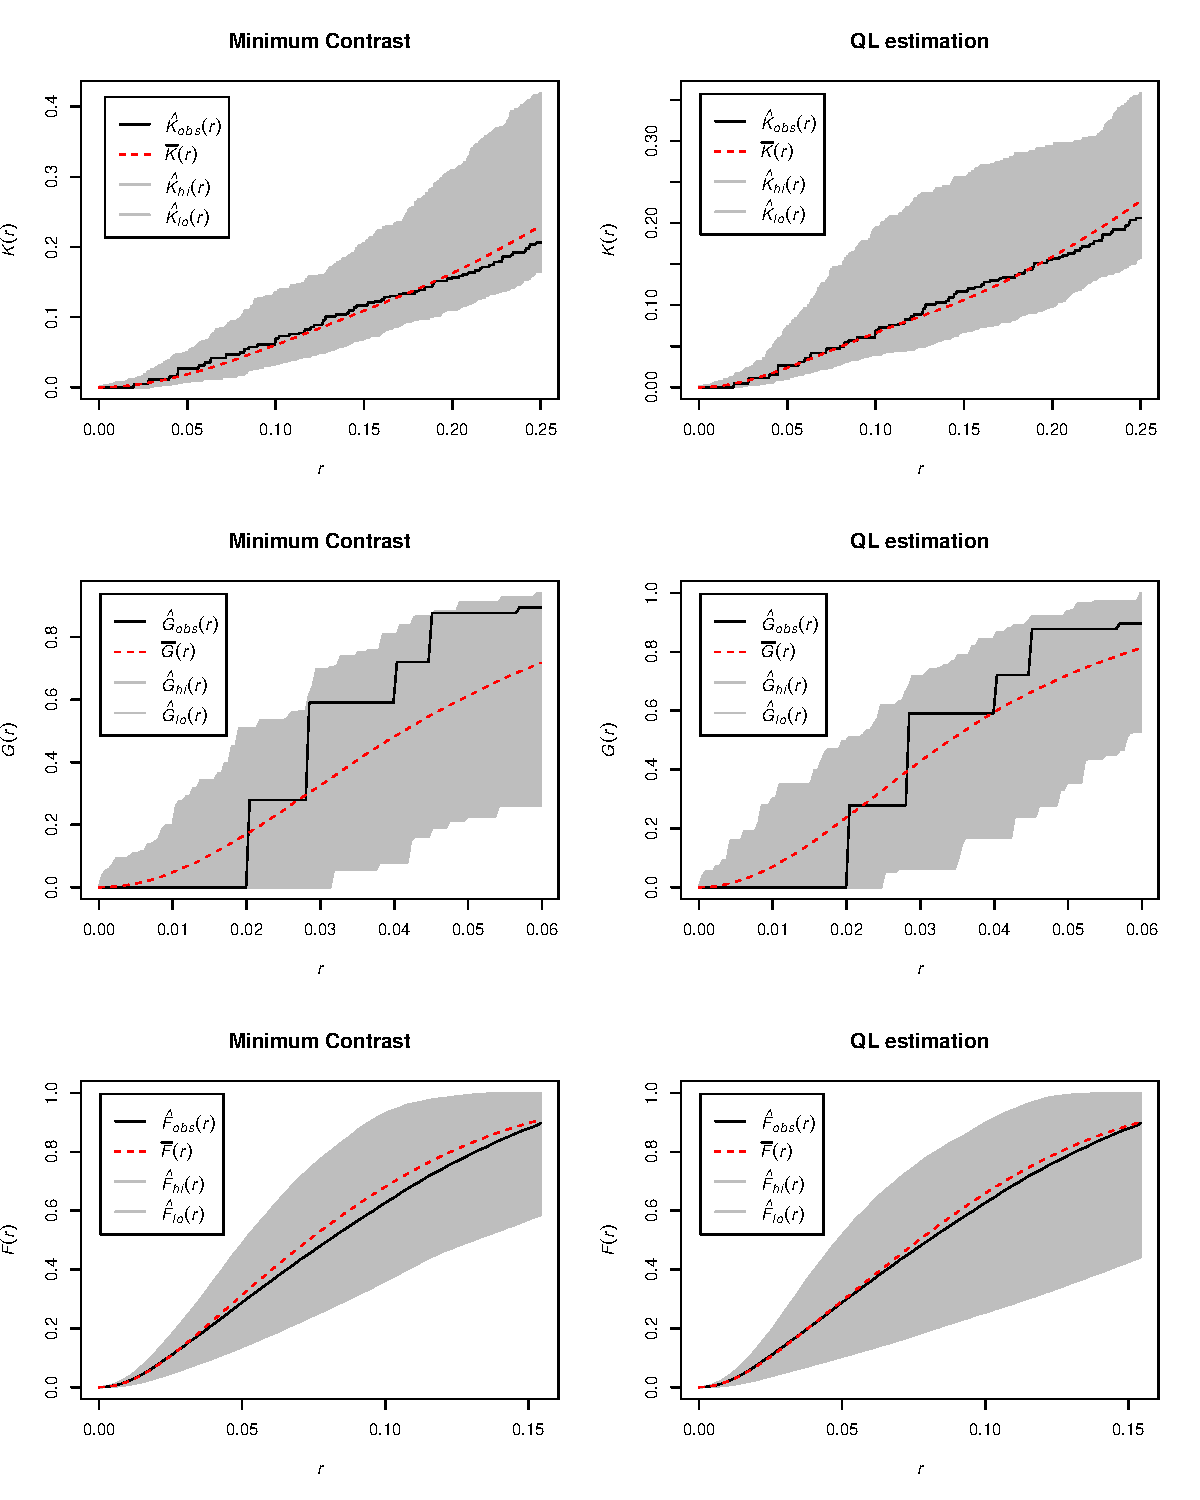
\includegraphics{Kfunc.pdf}
  \caption{Pointwise envelopes of the summary statistics $\hat{K}(r)$, $\hat{G}(r)$ and $\hat{F}(r)$
  based on simulated patterns of two fitted point process models for the
  \code{redwood} point pattern data: fitted by the method of minimum contrast
  (left column) and quasi-likelihood (right column).}
\label{fig:matclust}
\end{figure}
%
Finally, we compare the simulation envelopes based on the summary statistics
$\hat{K}$ and additionally $\hat{G}$ and $\hat{F}$. The plot in Figure
\ref{fig:matclust} suggests a good agreement between the model and the data for
both estimation methods with slightly better results by the quasi-likelihood
estimation approach regarding the envelopes of $\hat{G}$ and $\hat{F}$.
%%
\section{Conclusion}\label{sec:conclusion}
The package \pkg{qle} provides methods for parameter estimation for
a generic class of parametric statistical models. The estimation
approach is entirely simulation-based, in that moment characteristics of the
unknown distributions of the statistics are infered from model replications and
approximated by a specific kriging approach. Therefore, as a preliminary step,
the construction of the kriging approximations requires an experimental design
of randomly generated parameters or points. Also, users can assess its
predictive quality by error measures specifically tailored to the needs of the QL
estimation approach.\par
%
The estimation is based on finding a root of the QS vector but also subsumes
other estimation methods, e.\,g. simulated method of moments or least squares,
based on the Mahalanobis distance. Optionally, we could search for a suitable
starting parameter for our QL estimation approach by one of these methods first
because the corresponding criterion is potentially easier to compute and
minimize, particularly for small sample sizes, over the parameter space. Also we
can use gradient based and derivative-free methods, see package \pkg{nloptr}
\citep{pkg:nloptr}, for minimization of both criterion functions. On the
contrary, the quasi-scoring algorithm is solely used for root finding of the QS vector
in conjunction with the QD as a monitor function. Although the latter might
suffer from numerical instabilities due to sparsely sampled regions of the parameter space
(especially in the beginning of the estimation procedure in which case other
methods are employed automatically) it usually needs only a fraction of iterations compared
to other general purpose solvers.\par
%
In practice, it might be especially advantageous to (temporarily)
store or cache computational results of functions for a deeper analysis of
estimation results or even errors. Setting \code{options("qle.cache"=TRUE)}
persistently stores (and reloads) any results of the following functions:
\begin{itemize}
 \item[] \code{simQLdata}, \code{prefitCV}, \code{mahalDist}, \code{quasiDeviance},
 \item[] \code{fitCov}, \code{fitSIRFk}, \code{updateCovModels}, \code{getQLmodel}
\end{itemize}
using package \pkg{digest} \citep{pkg:digest} for hash digests of \proglang{R}
objects to create file names. Further, several options are available for
estimating the variance matrix of the statistics (e.\,g. using package \pkg{expm} \citep{pkg:expm}
for matrix logarithm transformations) as well as two types of prediction
variances (of sample mean values of statistics). These are used mainly in order to account for the
simulation error of the statistics while searching for potential candidates of the
unknown model parameter (either sampling from a multivariate normal based on the
package \pkg{mvtnorm} \citep{pkg:mvtnorm} or uniform distribution).
Finally, the user can perform a Monte Carlo hypothesis test in order to assess
the goodness-of-fit of the parametric model which does not involve additional simulations
(except for generating ''observations`` according to the fitted statistical model) and provides
predicted and empirically estimated standard errors of the model parameter.\par
%
\section{Computational details}
The package \pkg{qle} is implemented in \proglang{R} with extensions written in
\proglang{C/C++}. It can be found on the Comprehensive \proglang{R} Archive
Network at (CRAN, \url{http://CRAN.R-project.org/package=qle}) and also is hosted on
R-Forge at (\url{http://r-forge.r-project.org/projects/qle}). It uses a
NAMESPACE and depends on the package \pkg{parallel} \citep{pkg:stats} and
\pkg{nloptr} \citep{pkg:nloptr} among others (see above). To reproduce the
examples of the vignette, which are also provided as separate \proglang{R}
source files, we recommend the package \pkg{spatstat}.\par
%
Many functions, where appropriate, include the option to be used in a parallel
environment (based on the package \pkg{parallel}) either by spawning tasks to multiple
cores of a single system (see \code{mclapply}\footnote{Note that \code{mclapply}
is not available on Windows systems due to OS limitations.
Instead, it is strongly recommended to use a local cluster object (see
\code{makeCluster}).} for details) or distributing the tasks to a
multi-processor cluster. This mostly reduces the computational overhead produced by auxiliary
computational tasks. The package \pkg{qle} automatically compiles when
installed. The current version used for the examples of this vignette is 0.16-5.
%
\section*{Acknowledgments}
The authors would like to thank the German Science Foundation (DFG) for financial support of
this research within the framework of the priority program ''Life$\infty$``
(SPP 1466).
%
\bibliography{qlebib}
\end{document}
